%!TEX root = ../main.tex
\chapter{Onde elettromagnetiche}

In generale si definisce come onda una qualsiasi perturbazione, impulsiva o periodica, rispetto ai valori di equilibrio di un campo che descrive una proprietà di un sistema fisico, la quale si propaghi a velocità ben determinata.

Ricordiamo che con campo intendiamo una grandezza fisica che può essere definita in ogni istante in ciascun punto dello spazio e si può trattare di una grandezza vettoriale o scalare. La temperatura, la pressione, la densità di un fluido, pensato come un mezzo continuo, sono esempi già incontrati di campi. Essi sono scalari perché basta una sola funzione per definirli completamente: il valore del campo in un punto $(x,y,z)$ in un certo istante $t$ è quindi un numero. Il campo elettrico e il campo magnetico nel vuoto o in mezzi materiali sono esempi di campi vettoriali, per definirli in un dato sistema cartesiano occorrono tre funzioni. Un'onda elastica in un oggetto (una sbarra, ad esempio) è una deformazione locale, rappresentabile con uno spostamento dalla posizione di equilibrio di una sezione della sbarra e con una variazione di pressione, che si propaga lungo la sbarra stessa. Un'onda sonora è una perturbazione dello stato di equilibrio della pressione e della densità che si propaga in un gas. Le onde elettromagnetiche sono la perturbazione di un campo elettrico o di un campo magnetico, prodotta da cariche in moto, che si propagano nello spazio circostante. Esse vengono descritte in forma vettoriale ma il campo elettromagnetico ha una struttura più complessa, di carattere tensoriale.

La perturbazione di un campo che, prodotta da una sorgente, si propaga nello spazio, viene rappresentata con la funzione $\xi(x,y,z,t)$, detta funzione d'onda. Una situazione particolare è costituita dalle cosiddette onde piane, descritte dalla funzione $\xi(x,t)$, spazialmente unidimensionale, cioè dipendenti dalla sola coordinata spaziale $x$ oltre che dal tempo. Il nome di onda piana deriva dal fatto che la perturbazione in un certo istante $t_0$ assume lo stesso valore $\xi(x_0,t_0)$ in tutti i punti del piano di equazione $x=x_0$, ortogonale all'asse di propagazione $x$.

\[
	f=(\vec{r},t) = f(x,t)
\]

Supporremo che la forma della perturbazione (profilo dell'onda) rimanga inalterata durante la propagazione.
Si verifica che sono possibili solo due forme generali di propagazione:

\begin{itemize}
	\item \textbf{onda progressiva}, descritta da una $f(x,t)$ data da:
	\[
		f_p(x,t)=\xi(x-vt)
	\]
	\item \textbf{onda regressiva}, descritta da $f(x,t)$ data da:
	\[
		f_r(x,t)=\xi(x+vt)
	\]
\end{itemize}

\begin{figure}[htpb]
	\centering

	\tikzset{every picture/.style={line width=0.75pt}} %set default line width to 0.75pt        

	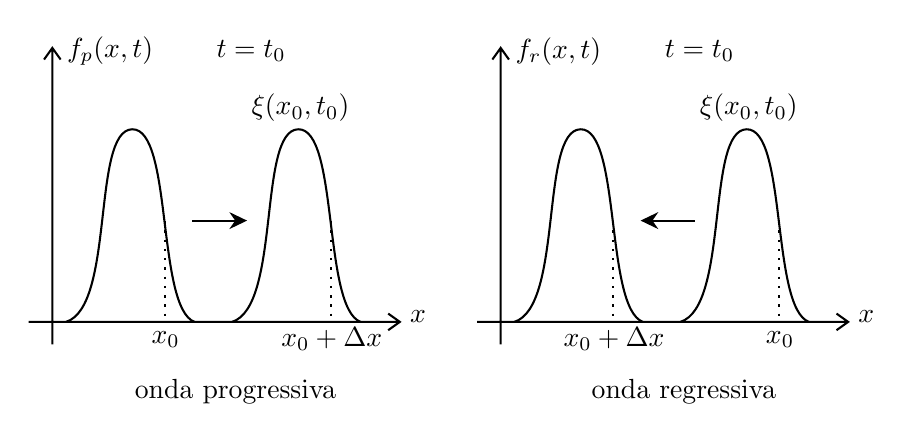
\begin{tikzpicture}[x=0.75pt,y=0.75pt,yscale=-0.8,xscale=0.8]
	%uncomment if require: \path (0,348); %set diagram left start at 0, and has height of 348

	%Shape: Axis 2D [id:dp43615178825650913] 
	\draw  (66.5,242) -- (290,242)(80.73,77) -- (80.73,255.5) (283,237) -- (290,242) -- (283,247) (75.73,84) -- (80.73,77) -- (85.73,84)  ;
	%Curve Lines [id:da6912254946371756] 
	\draw    (89,242) .. controls (118.46,232.67) and (104.33,126.67) .. (128.77,126) .. controls (153.21,125.33) and (143.5,233.33) .. (166.33,242) ;
	%Curve Lines [id:da055272540593983566] 
	\draw    (189,242) .. controls (218.46,232.67) and (204.33,126.67) .. (228.77,126) .. controls (253.21,125.33) and (243.5,233.33) .. (266.33,242) ;
	%Straight Lines [id:da676398524434098] 
	\draw  [dash pattern={on 0.84pt off 2.51pt}]  (148.33,181.25) -- (148.33,242) ;
	%Straight Lines [id:da3877990784406371] 
	\draw  [dash pattern={on 0.84pt off 2.51pt}]  (248.33,181.25) -- (248.33,242) ;
	%Straight Lines [id:da3894091384014513] 
	\draw    (165,181) -- (195,181) ;
	\draw [shift={(198,181)}, rotate = 180] [fill={rgb, 255:red, 0; green, 0; blue, 0 }  ][line width=0.08]  [draw opacity=0] (10.72,-5.15) -- (0,0) -- (10.72,5.15) -- (7.12,0) -- cycle    ;
	%Shape: Axis 2D [id:dp9772982264856409] 
	\draw  (336.5,242) -- (560,242)(350.73,77) -- (350.73,255.5) (553,237) -- (560,242) -- (553,247) (345.73,84) -- (350.73,77) -- (355.73,84)  ;
	%Curve Lines [id:da9272160229851911] 
	\draw    (359,242) .. controls (388.46,232.67) and (374.33,126.67) .. (398.77,126) .. controls (423.21,125.33) and (413.5,233.33) .. (436.33,242) ;
	%Curve Lines [id:da8269961796909089] 
	\draw    (459,242) .. controls (488.46,232.67) and (474.33,126.67) .. (498.77,126) .. controls (523.21,125.33) and (513.5,233.33) .. (536.33,242) ;
	%Straight Lines [id:da5013690882799777] 
	\draw  [dash pattern={on 0.84pt off 2.51pt}]  (418.33,181.25) -- (418.33,242) ;
	%Straight Lines [id:da3290243185281636] 
	\draw  [dash pattern={on 0.84pt off 2.51pt}]  (518.33,181.25) -- (518.33,242) ;
	%Straight Lines [id:da27607590836085505] 
	\draw    (438,181) -- (468,181) ;
	\draw [shift={(435,181)}, rotate = 0] [fill={rgb, 255:red, 0; green, 0; blue, 0 }  ][line width=0.08]  [draw opacity=0] (10.72,-5.15) -- (0,0) -- (10.72,5.15) -- (7.12,0) -- cycle    ;

	% Text Node
	\draw (115.5,79) node    {$f_{p}( x,t)$};
	% Text Node
	\draw (200.5,79) node    {$t=t_{0}$};
	% Text Node
	\draw (230.17,113.17) node    {$\xi ( x_{0} ,t_{0})$};
	% Text Node
	\draw (149,252.5) node    {$x_{0}$};
	% Text Node
	\draw (249,252.5) node    {$x_{0} +\Delta x$};
	% Text Node
	\draw (301,239) node    {$x$};
	% Text Node
	\draw (385.5,79) node    {$f_{r}( x,t)$};
	% Text Node
	\draw (470.5,79) node    {$t=t_{0}$};
	% Text Node
	\draw (500.17,113.17) node    {$\xi ( x_{0} ,t_{0})$};
	% Text Node
	\draw (419,252.5) node    {$x_{0} +\Delta x$};
	% Text Node
	\draw (519,252.5) node    {$x_{0}$};
	% Text Node
	\draw (571,239) node    {$x$};
	% Text Node
	\draw (191,284) node   [align=left] {onda progressiva};
	% Text Node
	\draw (461,284) node   [align=left] {onda regressiva};

	\end{tikzpicture}
\end{figure}
\FloatBarrier

L'argomento di $\xi$ deve quindi contenere le variabili $x$ e $t$ sotto forma di combinazione lineare. Si tratta di una condizione sull'argomento. La funzione può poi assumere qualsiasi forma.

\textbf{Caso dell'onda progressiva}
Attendiamo un certo $ \Delta t $ e facciamo propagare l'onda. Dobbiamo vedere qual è il legame fra $ \Delta x $ e $ \Delta t $. Sfruttiamo il fatto che il valore assunto dalla funzione all'istante $t_0 $ nella posizione $x_0$ si ritrova in qualsiasi istante successivo che soddisfi la condizione:

\begin{gather*}
	f_p(x_0,t_0) = f_p(x_0+\Delta x,t_0+\Delta t) \\
	\xi(x_0-v\,t_0) = \xi(x_0+\Delta x-v\,t_0-v\Delta t) \\
	\Delta x - v\Delta t = 0 \\
	v = \frac{\Delta x}{\Delta t}
\end{gather*}

Si ottiene tale relazione che indica un moto rettilineo lungo l'asse $x$ con velocità $v$.

\textbf{Caso dell'onda regressiva}
Possiamo fare un discorso analogo per le onde regressive e scrivere:

\begin{gather*}
	f_r(x_0,t_0) = f_r(x_0+\Delta x,t_0+\Delta t) \\
	\xi(x_0+v\,t_0) = \xi(x_0+\Delta x + v\,t_0 + v\Delta t) \\
	\Delta x + v\Delta t = 0 \\
	v = - \frac{\Delta x}{\Delta t}
\end{gather*}

Analogamente ritroviamo che la funzione rappresenta una grandezza che si propaga con velocità $v$ lungo il verso negativo dell'asse $x$.
In entrambi i casi si tratta di una traslazione rigida, nel senso che la funzione non cambia mai forma.
Vogliamo trovare un equazione delle onde che descriva qualunque fenomeno ondulatorio. Una qualsiasi equazione ondulatoria deve obbedire all'\textbf{equazione delle onde} o \textbf{di d'Alembert} che nel caso di onda piana assume la seguente forma semplificata:

\[
	\frac{\partial^2 \xi}{\partial x^2}  - \frac{1}{v^2} \frac{\partial^2 \xi}{\partial t^2} = 0
\]
è semplice verificare che $ \xi(x\pm vt) $ è soluzione dell'equazione di d'Alembert. A tal proposito, occorre introdurre la variabile ausiliaria $ \eta = x \pm vt $

\begin{gather*}
	\frac{\partial \xi}{\partial x} = \frac{\partial \xi}{\partial \eta} \cdot \frac{\partial \eta}{\partial \xi} = \frac{\partial \xi}{\partial \eta}\\
	\frac{\partial^2 \xi}{\partial x^2} = \frac{\partial}{\partial x} \left[ \frac{\partial \xi}{\partial \eta}  \right] = \frac{\partial}{\partial \eta} \left[ \frac{\partial \xi}{\partial \eta}  \right] \cdot \frac{\partial \eta}{\partial x} = \frac{\partial^2 \xi}{\partial \eta^2}
\end{gather*}

E poi

\begin{gather*}
	\frac{\partial \xi}{\partial t} = \frac{\partial \xi}{\partial \eta} \cdot \frac{\partial \eta}{\partial t} = \frac{\partial \xi}{\partial \eta} (\pm v)\\
	\frac{\partial^2 \xi}{\partial t^2} = \frac{\partial}{\partial t} \left[ (\pm v)\frac{\partial \xi}{\partial \eta}  \right] = \frac{\partial}{\partial \eta} \left[ (\pm )\frac{\partial \xi}{\partial \eta}  \right] \cdot \frac{\partial \eta}{\partial t} = \frac{\partial^2 \xi}{\partial \eta^2} (\pm v)^2
\end{gather*}

Da cui

\[
	\frac{\partial^2 \xi}{\partial t^2} = v^2 \frac{\partial^2 \xi}{\partial x^2} \implies \boxed{\frac{\partial^2 \xi}{\partial x^2} -\frac{1}{v^2}\frac{\partial^2 \xi}{\partial t^2} = 0}
\]

\section{Onde piane armoniche (o sinusoidali)}

Un tipo particolare di onda piana è l'onda sinusoidale, o armonica. Le onde sinusoidali sono quelle per cui la funzione è un seno o un coseno; vengono percepite dall'occhio umano con un colore ben preciso e prendono per questo il nome di onde monocromatiche. La loro funzione d'onda si scrive come

\[
	\xi(x,t) = \xi_0 \sin [k(x-vt)] \qquad \xi(x,t) = \xi_0 \cos [k(x-vt)]
\]
$k$ prende il nome di \textbf{numero d'onda} e viene inserita per ragioni dimensionali in quanto l'argomento di un seno o di un coseno deve essere espresso in radianti. Possiamo riscrivere l'equazione come:

\[
	\xi(x,t) = \xi_0 \sin [kx - \underbrace{kv}_{\omega} t] = \xi_0 \sin [kx - \omega t]
\]
$kv$ viene chiamato pulsazione dell'onda, $\omega$. Se fissiamo un certo istante temporale $t_0 $ e facciamo un grafico dell'andamento della funzione, vedremo un andamento sinusoidale. La distanza lungo l'asse $x$ fra due punti che assumono lo stesso valore prende il nome di \textbf{lunghezza d'onda} $\lambda$ e ci dà la sua periodicità spaziale. Possiamo legare $\lambda$ con $k$ con la relazione:

\[
	\lambda = \frac{2\pi}{k}
\]

Si deduce che $k$ è uguale al numero di lunghezze d'onda che stanno su una distanza pari a $ 2\pi  $ metri. Se invece fissiamo una certa posizione, la $ \xi(x_0,t) $ dà la variazione nel tempo della funzione d'onda. Parleremo di \textbf{periodo} invece che di lunghezza d'onda. Si tratta dell'intervallo di tempo che separa due istanti successivi in cui la funzione assume lo stesso valore.

\[
	T = \frac{2\pi}{\omega}
\]

Definiamo anche la \textbf{frequenza} come l'inverso del periodo: $ \nu = \frac{1}{T} $. Si trova quindi che i due periodi, spaziale e temporale, sono legati dalla relazione

\[
	\nu = \frac{\omega}{2\pi} = \frac{kv}{2\pi} = \frac{v}{\lambda} \implies v = \lambda\nu \quad \lambda = vT
\]

L'onda in un periodo $T$ alla velocità $v$ percorre una distanza pari alla lunghezza d'onda.
Nel seguito dovremo spesso considerare onde armoniche del tipo:

\[
	\xi = \xi_0 \sin [\underbrace{kx-\omega t + \varphi}_{\text{fase dell'onda}}]
\]

Tutto l'argomento del seno è detto fase dell'onda sinusoidale. La fase ci consente di trovare un modo per visualizzare com'è fatta un onda. Infatti, fissato l'istante $t$, la superficie in cui la fase è costante prende il nome di \textbf{fronte d'onda} o fronte di fase.

\[
	\Phi (x_0, t_0) = \text{costante}
\]

Per un'onda piana il fronte d'onda è un piano o quanto meno una porzione di piano. Esso si sposta con la velocità $v$ di propagazione dell'onda.

\begin{figure}[htpb]
	\centering

	\tikzset{every picture/.style={line width=0.75pt}} %set default line width to 0.75pt        

	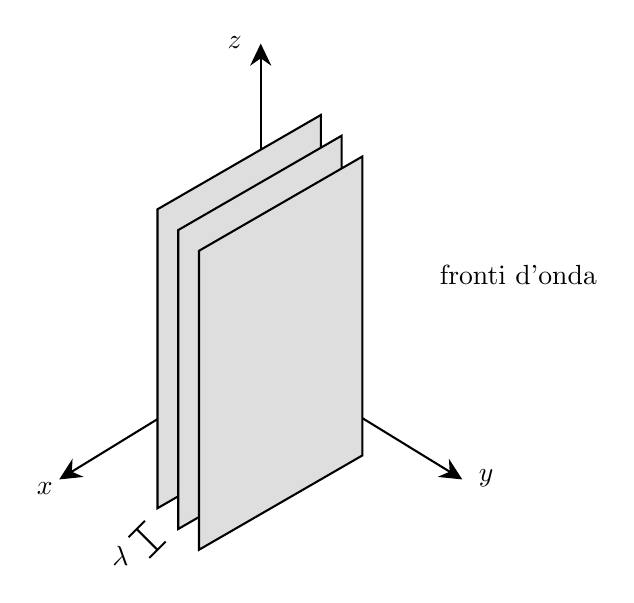
\begin{tikzpicture}[x=0.75pt,y=0.75pt,yscale=-1,xscale=1]
	%uncomment if require: \path (0,300); %set diagram left start at 0, and has height of 300

	%Straight Lines [id:da4035621045003759] 
	\draw    (276.9,162.92) -- (371.44,220.93) ;
	\draw [shift={(374,222.5)}, rotate = 211.53] [fill={rgb, 255:red, 0; green, 0; blue, 0 }  ][line width=0.08]  [draw opacity=0] (10.72,-5.15) -- (0,0) -- (10.72,5.15) -- (7.12,0) -- cycle    ;
	%Straight Lines [id:da4284318663584288] 
	\draw    (276.9,162.92) -- (276.9,15.5) ;
	\draw [shift={(276.9,12.5)}, rotate = 450] [fill={rgb, 255:red, 0; green, 0; blue, 0 }  ][line width=0.08]  [draw opacity=0] (10.72,-5.15) -- (0,0) -- (10.72,5.15) -- (7.12,0) -- cycle    ;
	%Straight Lines [id:da09535241990565257] 
	\draw    (276.9,162.92) -- (182.36,220.93) ;
	\draw [shift={(179.8,222.5)}, rotate = 328.47] [fill={rgb, 255:red, 0; green, 0; blue, 0 }  ][line width=0.08]  [draw opacity=0] (10.72,-5.15) -- (0,0) -- (10.72,5.15) -- (7.12,0) -- cycle    ;
	%Shape: Rectangle [id:dp0706669936577331] 
	\draw  [fill={rgb, 255:red, 222; green, 222; blue, 222 }  ,fill opacity=1 ] (305.9,46.89) -- (305.9,190.92) -- (227.15,236.39) -- (227.15,92.36) -- cycle ;
	%Shape: Rectangle [id:dp28618755049087685] 
	\draw  [fill={rgb, 255:red, 222; green, 222; blue, 222 }  ,fill opacity=1 ] (315.9,56.89) -- (315.9,200.92) -- (237.15,246.39) -- (237.15,102.36) -- cycle ;
	%Shape: Rectangle [id:dp8603680037835846] 
	\draw  [fill={rgb, 255:red, 222; green, 222; blue, 222 }  ,fill opacity=1 ] (325.9,66.89) -- (325.9,210.92) -- (247.15,256.39) -- (247.15,112.36) -- cycle ;
	%Straight Lines [id:da3406983498207887] 
	\draw    (217.15,246.39) -- (227.15,256.39) ;
	\draw [shift={(227.15,256.39)}, rotate = 225] [color={rgb, 255:red, 0; green, 0; blue, 0 }  ][line width=0.75]    (0,5.59) -- (0,-5.59)   ;
	\draw [shift={(217.15,246.39)}, rotate = 225] [color={rgb, 255:red, 0; green, 0; blue, 0 }  ][line width=0.75]    (0,5.59) -- (0,-5.59)   ;

	% Text Node
	\draw (172.87,226.84) node    {$x$};
	% Text Node
	\draw (385.47,221.75) node    {$y$};
	% Text Node
	\draw (264.29,12.16) node    {$z$};
	% Text Node
	\draw (401,124) node   [align=left] {fronti d'onda};
	% Text Node
	\draw (209.37,259.34) node    {$\lambda $};

	\end{tikzpicture}
\end{figure}
\FloatBarrier

Può infine convenire descrivere le funzioni d'onda come le formule di Eulero.

\begin{equation*}
	\begin{aligned}
		\xi(x,t) &= \xi_0\cos [kx-\omega t+\varphi] = \xi_0\cos [\Phi (x,t)] \\
		&= \frac{\xi_0}{2} [e^{i\Phi (x,t)} + e^{-i\Phi (x,t)}] \\
		&= \frac{\xi_0}{2} [e^{i\Phi (x,t)} + \text{complesso congiugato} ]
	\end{aligned}
\end{equation*}

\section{Onde longitudinali, onde trasversali, polarizzazione}

Un'onda piana è caratterizzata da un'unica direzione di propagazione, che per semplicità abbiamo indicato con l'asse $x$. Se tutte le grandezze significative relative
alla perturbazione che si propaga hanno direzione di
variazione che coincide con l'asse $x$, l'onda si dice longitudinale. L'onda acustica ne è un esempio. La pressione infatti non cambia in direzione perpendicolare a quella dell'onda ma nella direzione stessa di propagazione.
Invece in una corda tesa la direzione di propagazione è quella della corda ma il campo varia in direzione ortogonale ad essa. Quando la direzione di variazione dl campo è ortogonale alla direzione di variazione dell'onda, parleremo di onda trasversale. In questo caso non possiamo più rappresentare l'onda con una funzione scalare perché dobbiamo specificare la direzione in cui varia il campo. Dunque dobbiamo proiettare il vettore nel piano ortogonale alla direzione di propagazione. In una qualunque onda trasversale, fissati arbitrariamente gli assi $y$ e $z$ in un piano ortogonale all'asse $x$, la funzione d'onda è rappresentabile come un vettore $\xi$ le cui componenti sono in direzione $y$ e $z$. Visto che c'è questo ulteriore grado di libertà si possono verificare diverse situazioni. La direzione di variazione, ad esempio, può essere una qualsiasi delle infinite perpendicolari alla direzione di propagazione.
Potrebbe accadere che il vettore $\xi$ cambi casualmente nel tempo. Parleremo di \textbf{onda trasversale non polarizzata}. Se esiste una legge che ci dice come varia il versore nel tempo, parleremo di \textbf{onda polarizzata}. Le onde armoniche sono sempre polarizzate.

\paragraph{Onde piane sinusoidali trasversali.} Esse si rappresentano come:

\begin{gather*}
	\vec{\xi} (x,t) = \xi_z (x,t) \vec{u}_z + \xi_y (x,t) \vec{u}_y \\
	\xi_z = \xi_{0z}\sin (kx-\omega t) \qquad \xi_y = \xi_{0y}\sin (kx-\omega t + \delta )
\end{gather*}

In cui $\delta$ rappresenta la differenza di fase tra le due onde componenti. Le ampiezze $\xi_{0z}$, $\xi_{0y}$ insieme a $\delta$ permettono di conoscere ovunque e in ogni istante la funzione d'onda $\xi$. Esaminiamo alcuni casi in cui la differenza di fase ha valore costante.

Se $ \delta = 0 $ in ogni punto dell'asse $x$ e in ogni istante il vettore d'onda $\xi$ ha direzione fissa, formante con l'asse $y$ l'angolo $ \vartheta  $. Se $ \delta = \pi $ (componenti dell'onda in opposizione di fase), la situazione è la stessa, solo che la direzione di $\xi$ è opposta.

\begin{figure}[htpb]
	\centering

	\tikzset{every picture/.style={line width=0.75pt}} %set default line width to 0.75pt        

	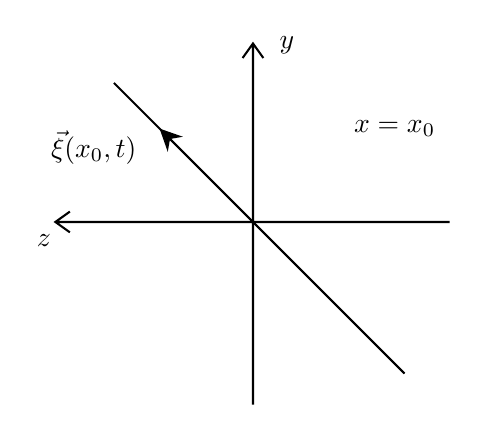
\begin{tikzpicture}[x=0.75pt,y=0.75pt,yscale=-1,xscale=1]
	%uncomment if require: \path (0,300); %set diagram left start at 0, and has height of 300

	%Shape: Axis 2D [id:dp1578987810426533] 
	\draw  (398.5,153) -- (208.5,153)(303.71,67) -- (303.71,241) (215.5,148) -- (208.5,153) -- (215.5,158) (308.71,74) -- (303.71,67) -- (298.71,74)  ;
	%Straight Lines [id:da9166949085494358] 
	\draw    (236.71,86) -- (376.71,226) ;
	%Straight Lines [id:da1792511694869101] 
	\draw    (260.83,110.12) -- (376.71,226) ;
	\draw [shift={(258.71,108)}, rotate = 45] [fill={rgb, 255:red, 0; green, 0; blue, 0 }  ][line width=0.08]  [draw opacity=0] (10.72,-5.15) -- (0,0) -- (10.72,5.15) -- (7.12,0) -- cycle    ;

	% Text Node
	\draw (227,117) node    {$\vec{\xi }( x_{0} ,t)$};
	% Text Node
	\draw (320,68) node    {$y$};
	% Text Node
	\draw (203,162) node    {$z$};
	% Text Node
	\draw (372,108) node    {$x=x_{0}$};

	\end{tikzpicture}
\end{figure}
\FloatBarrier

Quando il vettore $\xi$ ha direzione fissa si dice che l'onda piana è \textbf{polarizzata linearmente} o rettilinearmente. La direzione fissa di $\xi$ è chiamata \textbf{direzione di polarizzazione} e il piano fisso su cui essa giace è detto \textbf{piano di polarizzazione}. Poniamo ora $ \delta =\frac{\pi}{2} $. Si avrà:

\[
	\xi_z = \xi_{0z} \cos (kx-\omega t) \qquad \xi_y = \xi_{0y}\sin (kx-\omega t)
\]

Si tratta di due sinusoidi in quadratura di fase. Se ci poniamo in un punto $x=x_0$, siccome le due componenti oscillano in modo sfasato, il vettore avrà andamento ellittico in funzione del tempo. Le componenti dell'onda infatti soddisfano l'equazione:

\[
	\frac{\xi_y^2}{\xi_{0y}^2} + \frac{\xi_z^2}{\xi_{0z}^2} = 1
\]

Al passare del tempo si vede la punta di $\xi$ descrivere un'ellisse.
Per $ \frac{3}{2} \pi  $ cambia il verso in cui l'elica gira, da orario a antiorario. Si parla di onda \textbf{polarizzata ellitticamente}.

\begin{figure}[htpb]
	\centering

	\tikzset{every picture/.style={line width=0.75pt}} %set default line width to 0.75pt        

	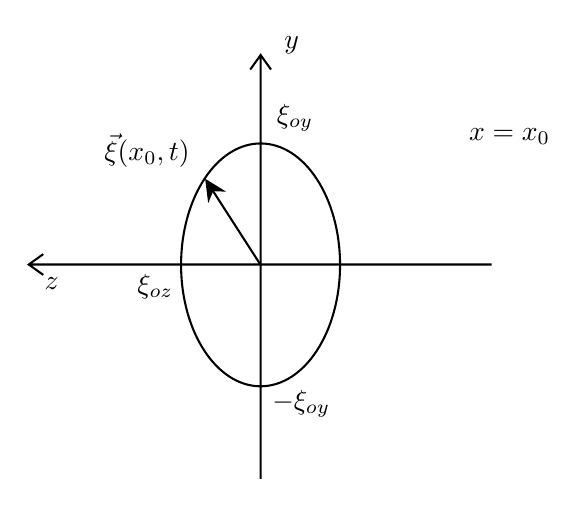
\begin{tikzpicture}[x=0.75pt,y=0.75pt,yscale=-1,xscale=1]
	%uncomment if require: \path (0,300); %set diagram left start at 0, and has height of 300

	%Shape: Axis 2D [id:dp4786260302496421] 
	\draw  (435,172.83) -- (212,172.83)(323.74,71.89) -- (323.74,276.11) (219,167.83) -- (212,172.83) -- (219,177.83) (328.74,78.89) -- (323.74,71.89) -- (318.74,78.89)  ;
	%Straight Lines [id:da6430509685027268] 
	\draw    (298.62,134.02) -- (323.71,173) ;
	\draw [shift={(297,131.5)}, rotate = 57.24] [fill={rgb, 255:red, 0; green, 0; blue, 0 }  ][line width=0.08]  [draw opacity=0] (10.72,-5.15) -- (0,0) -- (10.72,5.15) -- (7.12,0) -- cycle    ;
	%Shape: Ellipse [id:dp03331606762220707] 
	\draw   (285.41,173) .. controls (285.41,140.69) and (302.56,114.5) .. (323.71,114.5) .. controls (344.86,114.5) and (362,140.69) .. (362,173) .. controls (362,205.31) and (344.86,231.5) .. (323.71,231.5) .. controls (302.56,231.5) and (285.41,205.31) .. (285.41,173) -- cycle ;

	% Text Node
	\draw (269,118) node    {$\vec{\xi }( x_{0} ,t)$};
	% Text Node
	\draw (338.67,67.33) node    {$y$};
	% Text Node
	\draw (223,182) node    {$z$};
	% Text Node
	\draw (443.67,111) node    {$x=x_{0}$};
	% Text Node
	\draw (340.33,102) node    {$\xi _{oy}$};
	% Text Node
	\draw (343.33,240) node    {$-\xi _{oy}$};
	% Text Node
	\draw (273,183.33) node    {$\xi _{oz}$};

	\end{tikzpicture}
\end{figure}
\FloatBarrier

Se le due ampiezze sono uguali l'ellisse diventa un cerchio. Parleremo di \textbf{polarizzazione circolare}, caso particolare della polarizzazione ellittica

\[
	\xi_{0y} = \xi_{0z}
\]

Se $\delta$ non è uno dei quattro angoli citati ($0$, $ \pi  $, $ \frac{\pi}{2} $, $ \frac{3\pi}{2} $) si parla di \textbf{onda polarizzata ellitticamente ma con assi ruotati} rispetto a $y$ e $z$.

\section{Onde in più dimensioni}

Vediamo quale sarebbe la forma più generale, se la direzione di propagazione fosse generica. Chiameremo $x'$ l'asse in cui l'onda propaga. Vogliamo esprimere la funzione che rappresenta l'andamento sinusoidale in un sistema di coordinate differente. Sia $\vec{r}$ il raggio-vettore che individua un punto $P$ di un certo fronte d'onda piano.

\begin{figure}[htpb]
	\centering

	\tikzset{every picture/.style={line width=0.75pt}} %set default line width to 0.75pt        

	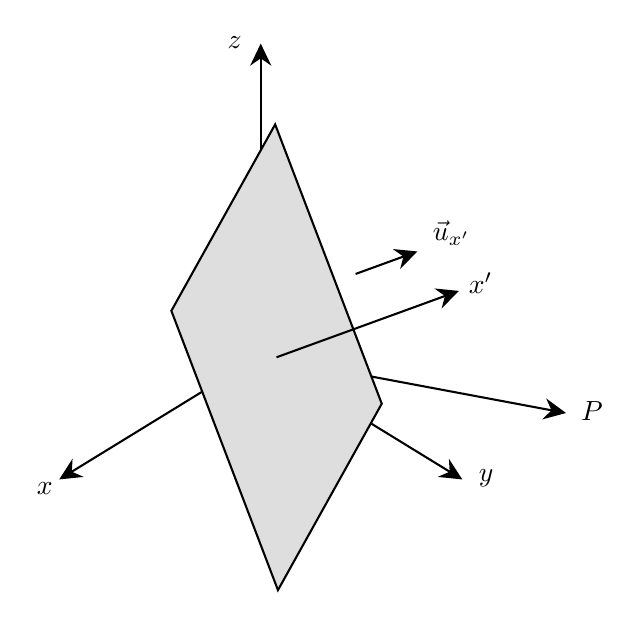
\begin{tikzpicture}[x=0.75pt,y=0.75pt,yscale=-1,xscale=1]
	%uncomment if require: \path (0,300); %set diagram left start at 0, and has height of 300

	%Straight Lines [id:da9506068607557134] 
	\draw    (296.9,182.92) -- (441.05,209.95) ;
	\draw [shift={(444,210.5)}, rotate = 190.62] [fill={rgb, 255:red, 0; green, 0; blue, 0 }  ][line width=0.08]  [draw opacity=0] (10.72,-5.15) -- (0,0) -- (10.72,5.15) -- (7.12,0) -- cycle    ;
	%Straight Lines [id:da8959417063927446] 
	\draw    (296.9,182.92) -- (391.44,240.93) ;
	\draw [shift={(394,242.5)}, rotate = 211.53] [fill={rgb, 255:red, 0; green, 0; blue, 0 }  ][line width=0.08]  [draw opacity=0] (10.72,-5.15) -- (0,0) -- (10.72,5.15) -- (7.12,0) -- cycle    ;
	%Straight Lines [id:da9787666861777233] 
	\draw    (296.9,182.92) -- (296.9,35.5) ;
	\draw [shift={(296.9,32.5)}, rotate = 450] [fill={rgb, 255:red, 0; green, 0; blue, 0 }  ][line width=0.08]  [draw opacity=0] (10.72,-5.15) -- (0,0) -- (10.72,5.15) -- (7.12,0) -- cycle    ;
	%Straight Lines [id:da969195712272505] 
	\draw    (296.9,182.92) -- (202.36,240.93) ;
	\draw [shift={(199.8,242.5)}, rotate = 328.47] [fill={rgb, 255:red, 0; green, 0; blue, 0 }  ][line width=0.08]  [draw opacity=0] (10.72,-5.15) -- (0,0) -- (10.72,5.15) -- (7.12,0) -- cycle    ;
	%Shape: Rectangle [id:dp43868189433161064] 
	\draw  [fill={rgb, 255:red, 222; green, 222; blue, 222 }  ,fill opacity=1 ] (303.85,71.45) -- (355.21,206.01) -- (305.2,295.83) -- (253.84,161.27) -- cycle ;
	%Straight Lines [id:da4888413142571806] 
	\draw    (304.53,183.64) -- (389.54,152.7) ;
	\draw [shift={(392.36,151.67)}, rotate = 520] [fill={rgb, 255:red, 0; green, 0; blue, 0 }  ][line width=0.08]  [draw opacity=0] (10.72,-5.15) -- (0,0) -- (10.72,5.15) -- (7.12,0) -- cycle    ;
	%Straight Lines [id:da6230223655892035] 
	\draw    (342.61,143.5) -- (369.54,133.7) ;
	\draw [shift={(372.36,132.67)}, rotate = 520] [fill={rgb, 255:red, 0; green, 0; blue, 0 }  ][line width=0.08]  [draw opacity=0] (10.72,-5.15) -- (0,0) -- (10.72,5.15) -- (7.12,0) -- cycle    ;

	% Text Node
	\draw (192.87,246.84) node    {$x$};
	% Text Node
	\draw (405.47,241.75) node    {$y$};
	% Text Node
	\draw (284.29,32.16) node    {$z$};
	% Text Node
	\draw (402.87,147.84) node    {$x'$};
	% Text Node
	\draw (388.87,123.84) node    {$\vec{u}_{x'}$};
	% Text Node
	\draw (456.47,209.75) node    {$P$};

	\end{tikzpicture}
\end{figure}
\FloatBarrier

\begin{gather*}
	\xi(x',t) = \xi_0 \sin [kx'-\omega t] \\
	\vec{r} = x'\vec{u}_{x'}+y'\vec{u}_{y'}+z'\vec{u}_{z'} = x\vec{u}_x+y\vec{u}_y+z\vec{u}_z \\
\end{gather*}

Possiamo ottenere $ x' $ in funzione delle coordinate $ (x,y,z)  $ imponendo

\[
	x'=\vec{r} \cdot \vec{u}_{x'} = (x\vec{u}_x+y\vec{u}_y+z\vec{u}_z) \cdot  \vec{u}_{x'} = x\cos \alpha + y\cos \beta + z \cos \gamma
\]

Se moltiplichiamo per $k$ otteniamo l'espressione che sta nell'argomento del seno.

\[
	kx'=k\;\vec{r} \cdot \vec{u}_{x'} = \underbrace{k\,\vec{u}_{x'}}_{\vec{k}} \cdot \,\vec{r} = \vec{k} \cdot \vec{r}
\]

Abbiamo ottenuto un vettore che contiene due informazioni fondamentali riguardo l'onda:

\begin{itemize}
	\item Il numero d'onda
	\item Il verso di propagazione
\end{itemize}

Si tratta del vettore $ \vec{k}  $ che prende il nome di \textbf{vettore d'onda}. Possiamo esprimere in modo più generale un onda piana quando si propaga in una direzione generica dello spazio come:

\[
	\xi(x,y,z,t) = \xi_0\sin [\vec{k} \cdot \vec{r} -\omega t]
\]

L'invarianza del prodotto scalare assicura che questa espressione generale di onda armonica piana è indipendente dal sistema di coordinate prescelto per la sua descrizione analitica. Si dimostra che in questo caso l'onda di propagazione obbedisce alla seguente equazione di d'Alembert generale:

\[
	\frac{\partial^2 \xi}{\partial x^2} + \frac{\partial^2 \xi}{\partial y^2} + \frac{\partial^2 \xi}{\partial z^2} = \frac{1}{v^2} \frac{\partial^2 \xi}{\partial t^2} \implies \nabla^2 \xi = \frac{1}{v^2} \frac{\partial^2 \xi}{\partial t^2}
\]

\section{Onde elettromagnetiche}

Abbiamo visto che, nel caso di onde piane sinusoidali, l'espressione di $\xi$ è darà da:

\[
	\xi(\vec{r},t) = \xi_0\sin [\vec{k} \cdot \vec{r} -\omega t]
\]

Vogliamo adesso dimostrare come nelle equazioni di Maxwell siano in effetti contenuti fenomeni ondulatori e definire le onde elettromagnetiche nel più semplice caso di onda piana.

Consideriamo di trovarci in uno spazio vuoto nel quale non ci sono cariche libere e correnti di
conduzione. In queste ipotesi le equazioni di Maxwell hanno la forma

\begin{align}
	&\text{div}\vec{E} = 0 \\
	&\text{div}\vec{B} = 0 \\
	&\text{rot}\vec{E} = \frac{\partial \vec{B}}{\partial t} \\
	&\text{rot}\vec{B} = \mu_0 \varepsilon_0 \frac{\partial \vec{E}}{\partial t}
\end{align}

Proviamo ad applicare il rotore ad entrambe le parti della terza equazione

\begin{equation}
	\begin{aligned}
		\vec{\nabla} \times \left( \vec{\nabla} \times \vec{E} \right)   &= - \vec{\nabla} \times \left( \frac{\partial \vec{B}}{\partial t}  \right) \\
		\vec{\nabla} \underbrace{\left( \vec{\nabla} \cdot \vec{E} \right)}_{=0} - \nabla^2 \vec{E} &= - \frac{\partial}{\partial t} \underbrace{\left[\vec{\nabla} \times \vec{B} \right]}_{= \mu_0 \varepsilon_0 \frac{\partial \vec{E}}{\partial t}} \\
		\Aboxed{\nabla^2 \vec{E} &= \mu_0 \varepsilon_0 \frac{\partial^2 \vec{E}}{\partial t^2}}
	\end{aligned}
	\label{eq:maxwellElettrico}
\end{equation}

Analogamente, moltiplicando per il rotore entrambe le parti della quarta equazione:

\begin{equation}
	\begin{aligned}
		\vec{\nabla} \times \left( \vec{\nabla} \times \vec{B} \right)   &= \vec{\nabla} \times \left( \mu_0 \varepsilon_0 \frac{\partial \vec{E}}{\partial t}  \right) \\
		\vec{\nabla} \underbrace{\left( \vec{\nabla} \cdot \vec{B} \right)}_{=0} - \nabla^2 \vec{B} &= \mu_0 \varepsilon_0 \frac{\partial}{\partial t} \underbrace{\left[\vec{\nabla} \times \vec{E} \right]}_{= - \frac{\partial \vec{B}}{\partial t}} \\
		\Aboxed{\nabla^2 \vec{B} &= \mu_0 \varepsilon_0 \frac{\partial^2 \vec{B}}{\partial t^2}}
	\end{aligned}
	\label{eq:maxwellMagnetico}
\end{equation}

Le equazioni di Maxwell prevedono che i campi elettrici e magnetici possano propagarsi come delle onde; i risultati ottenuti infatti hanno forma analoga all'equazione di d'Alembert. Il risultato all'epoca risultò in contraddizione con le teorie esistenti perché prevedeva che le onde potessero propagarsi anche nel vuoto. Si pensava invece che la propagazione di esse dovesse sempre avvenire attraverso un mezzo, tant'è che furono condotti numerosi studi al fine di provare l'esistenza dell'\emph{etere luminifero}, ipotetico mezzo di trasmissione delle onde elettromagnetiche. Ne è un esempio l'esperimento (senza successo) di rilevare il movimento della terra attraverso l'etere di Michelson-Morley. È possibile calcolare la velocità di propagazione dell'onda come:

\[
	\frac{1}{c^2} = \mu_0 \varepsilon_0 \implies c = \frac{1}{\sqrt{\mu_0 \varepsilon_0}} \simeq 2,9979\ldots  \times 10^8 \,m/s
\]

Maxwell trovò questo valore della velocità $c$ (dal latino \emph{celeritas}) di propagazione delle onde elettromagnetiche, numero che era già stato individuato dall'apparato di Fizeau-Foucault (1849), un dispositivo per il calcolo della velocità della luce. Fu poi in seguito, grazie alle esperienze di Hertz, che fu definitivamente dimostrata la natura elettromagnetica dei fenomeni luminosi.
Sembrerebbe che fra i due campi non ci sia relazione, che possano esistere onde magnetiche o elettriche. Tuttavia se osserviamo le equazioni di Maxwell elencate all'inizio ci rendiamo conto di come la presenza di uno comporti la presenza dell'altro. Tale apparenza si ha perché nel momento in cui calcoliamo la derivata di una funzione (applicando il rotore) perdiamo informazioni sulle costanti.\\
\textbf{Osservazione}. Sostanzialmente le equazioni \eqref{eq:maxwellElettrico} e \eqref{eq:maxwellMagnetico} ci danno soluzioni per le onde elettromagnetiche, ma può capitare che alcune di esse non siano soluzioni delle equazioni di Maxwell, che vadano scartate. Abbiamo infatti perso informazioni sulla solenoidaleità dei campi.

In questo contesto si introduce l'\textbf{operatore d'alembertiano}, che viene indicato con un quadrato. Così come per il rotore viene utilizzato un triangolo, riferimento alle tre derivate spaziali, per tale operatore si hanno quattro lati che corrispondono alle coordinate $(x,y,z,t)$. Si ha una quarta coordinata spaziale, quella del tempo. Nella teoria della relatività si lavora con quattro dimensioni.

\[
	\boxed{\Box = \nabla^2 - \frac{1}{c^2} \frac{\partial^2}{\partial t^2}  \implies  \Box \vec{E} = 0 \quad \Box \vec{B} = 0}
\]
\textbf{Osservazione.} Se $\xi_1$ e $\xi_2$ sono soluzioni indipendenti dell'equazione di d'Alembert, per la sua linearità, anche la loro combinazione lineare lo è.

\[
	\xi = \xi_1a_1 + \xi_2a_2
\]

Supponiamo ora di avere un'onda piana che si propaga lungo l'asse $x$.

\[
	\vec{E} = E(x,t) \qquad \vec{B} = B(x,t)
\]

Questo comporta che la derivata rispetto a $y$ e $z$ di qualsiasi componente di questi vettori $\vec{B}$ ed $\vec{E}$ debba essere nulla. Applichiamo questa osservazione alle prime due equazioni di Maxwell:

\begin{equation*}
	\begin{aligned}
		\text{div}\vec{E} &= \frac{\partial E_x}{\partial x} + \frac{\partial E_y}{\partial y} + \frac{\partial E_z}{\partial z}  = 0 \implies \frac{\partial E_x}{\partial x} = 0 \\
		\text{div}\vec{B} &= \frac{\partial B_x}{\partial x} + \frac{\partial B_y}{\partial y} + \frac{\partial B_z}{\partial z}  = 0 \implies \frac{\partial B_x}{\partial x} = 0
	\end{aligned}
\end{equation*}

Consideriamo il rotore

\begin{equation*}
	\begin{aligned}
		\text{rot}\vec{E} &= \text{det} \begin{pmatrix}
		\vec{u}_x & \vec{u}_y & \vec{u}_z \\
		\frac{\partial}{\partial x}  &  \frac{\partial}{\partial y} & \frac{\partial}{\partial z} \\
		E_x & E_y & E_z
	\end{pmatrix} \\
	&= \vec{u}_x\left( \underbrace{\frac{\partial E_z}{\partial y}}_{=0} - \underbrace{\frac{\partial E_y}{\partial z}}_{=0}  \right) + \vec{u}_y \left( \underbrace{\frac{\partial E_x}{\partial z}}_{=0} - \frac{\partial E_z}{\partial x}  \right) + \vec{u}_z \left( \underbrace{\frac{\partial E_x}{\partial y}}_{=0} - \frac{\partial E_y}{\partial x}  \right)  \\
	&=-\frac{\partial \vec{B}}{\partial t} = - \vec{u}_x\frac{\partial B_x}{\partial t} - \vec{u}_y\frac{\partial B_y}{\partial t} - \vec{u}_z\frac{\partial B_z}{\partial t}
	\end{aligned}
\end{equation*}

Si ottiene

\begin{equation}
	\boxed{-\frac{\partial B_x}{\partial t} = 0 \qquad - \frac{\partial E_z}{\partial x} = - \frac{\partial B_y}{\partial t} \qquad \frac{\partial E_y}{\partial x} = - \frac{\partial B_z}{\partial t}}
	\label{eq:componenti1}
\end{equation}

Analogamente per il rotore di $\vec{B}$

\begin{equation*}
	\begin{aligned}
		\text{rot}\vec{B} &= \text{det} \begin{pmatrix}
		\vec{u}_x & \vec{u}_y & \vec{u}_z \\
		\frac{\partial}{\partial x}  &  \frac{\partial}{\partial y} & \frac{\partial}{\partial z} \\
		B_x & B_y & B_z
	\end{pmatrix} \\
	&= \vec{u}_x\left( \underbrace{\frac{\partial B_z}{\partial y}}_{=0} - \underbrace{\frac{\partial B_y}{\partial z}}_{=0}  \right) + \vec{u}_y \left( \underbrace{\frac{\partial B_x}{\partial z}}_{=0} - \frac{\partial B_z}{\partial x}  \right) + \vec{u}_z \left( \underbrace{\frac{\partial B_x}{\partial y}}_{=0} - \frac{\partial B_y}{\partial x}  \right)  \\
	&= \frac{1}{c^2}\frac{\partial \vec{E}}{\partial t} = \frac{1}{c^2} \vec{u}_x\frac{\partial E_x}{\partial t} + \frac{1}{c^2} \vec{u}_y\frac{\partial E_y}{\partial t} + \frac{1}{c^2} \vec{u}_z\frac{\partial E_z}{\partial t}
	\end{aligned}
\end{equation*}

Si ottiene

\begin{equation}
	\boxed{\frac{1}{c^2} \frac{\partial E_x}{\partial t} = 0 \qquad \frac{1}{c^2}\frac{\partial E_y}{\partial t} = - \frac{\partial B_z}{\partial x} \qquad \frac{1}{c^2} \frac{\partial E_z}{\partial t} = \frac{\partial B_y}{\partial x}}
	\label{eq:componenti2}
\end{equation}

Diamo una interpretazione ai risultati ottenuti.

\[
	\left. \begin{array}{r}
	 	\frac{\partial E_x}{\partial t} = 0 \\
		\frac{\partial E_x}{\partial t} = 0
	\end{array} \right\} \implies E_x = \text{costante} = 0
\]

\[
	\left. \begin{array}{r}
	 	\frac{\partial B_x}{\partial t} = 0 \\
		\frac{\partial B_x}{\partial t} = 0
	\end{array} \right\} \implies B_x = \text{costante} = 0
\]

Tali relazioni permettono di dire che le componenti $ E_x $ e $ B_x $ sono costanti. Un tale caso potrebbe essere prodotto da distribuzioni di cariche stazionarie (per $ \vec{E}  $) o da correnti stazionarie (per $ \vec{B}  $). Siccome escludiamo l'esistenza di sorgenti di questo tipo in quanto interessati ai campi variabili nel tempo, concludiamo che tali componenti sono nulle. Se la componente dei due campi lungo l'asse di propagazione è nullo significa che le onde elettromagnetiche sono trasversali. Osservando le altre 4 equazioni, si osserva un accoppiamento fra le componenti dei due campi fra loro ortogonali. Ci possiamo concentrare su una delle due modalità di oscillazione.

Ipotizziamo $ E_z = 0 $

\[
	\frac{\partial B_y}{\partial t} = 0 \quad \frac{\partial B_y}{\partial x} = 0 \implies B_y = \text{costante} = 0
\]

Derivando da entrambi i lati l'equazione ricavata precedentemente si ha:

\begin{equation*}
	\begin{aligned}
		\frac{\partial E_y}{\partial x} &= - \frac{\partial B_z}{\partial t} \\
		\frac{\partial}{\partial x} \left( \frac{\partial E_y}{\partial x}  \right) &= - \frac{\partial}{\partial x} \left( \frac{\partial B_z}{\partial t}  \right) \\
		\frac{\partial^2 E_y}{\partial x^2} &= - \frac{\partial^2 B_z}{\partial x \partial t}
	\end{aligned}
\end{equation*}

Poi

\begin{equation*}
	\begin{aligned}
		\frac{1}{c^2} \frac{\partial E_y}{\partial t} &= - \frac{\partial B_z}{\partial x} \\
		\frac{\partial}{\partial t} \left( \frac{1}{c^2} \frac{\partial E_y}{\partial t} \right) &= - \frac{\partial}{\partial t} \left( \frac{\partial B_z}{\partial x} \right) \\
		\frac{1}{c^2} \frac{\partial^2 E_y}{\partial t^2} &= - \frac{\partial^2 B_z}{\partial t\partial x}
	\end{aligned}
\end{equation*}

Uguagliando i due membri

\[
	\boxed{\frac{\partial^2 E_y}{\partial x^2} = \frac{1}{c^2} \frac{\partial^2 E_y}{\partial t^2}}
\]

Con conti analoghi, per $ \vec{B}$ si trova:

\[
	\boxed{\frac{\partial^2 B_z}{\partial x^2} = \frac{1}{c^2} \frac{\partial^2 B_z}{\partial t^2}}
\]

Con $ E_y = E_y(x-ct) $ e $ B_z  = B_z (x-ct) $
Vediamo come le due equazioni sono legate. Introduciamo la variabile ausiliaria $ \eta = x-ct $ e ricordiamo la terza equazione di \eqref{eq:componenti1}:

\begin{gather*}
	\frac{\partial E_y}{\partial x} = \frac{\partial E_y}{\partial \eta} \frac{\partial \eta}{\partial x} = \frac{\partial E_y}{\partial \eta} \qquad \frac{\partial B_z}{\partial t} = \frac{\partial B_z}{\partial \eta} \frac{\partial \eta}{\partial t} = (-c) \frac{\partial B_z}{\partial \eta} \\
	\frac{\partial E_y}{\partial \eta} = c \frac{\partial B_z}{\partial \eta} \implies E_y = c\,B_z + \text{costante}
\end{gather*}

Ponendo anche in questo caso a zero la costante, che descrive una situazione stazionaria alla quale non siamo interessati, ricaviamo

\[
	\boxed{E_y = c\,B_z}
\]

Ricaviamo la relazione vettoriale

\[
	\left. \begin{array}{r}
	 	E_y = E_y(x-ct) \\
		B_z = \frac{E_y}{c}(x-ct)
	\end{array} \right. \implies
	\left. \begin{array}{l}
	 	\vec{E} = E_y\vec{u}_y  \\
		\vec{B} = \frac{E_y}{c} \vec{u}_z
	\end{array} \right.
\]

Vista la relazione fra le componenti, possiamo scrivere direttamente $\vec{E}$ come:

\[
	\boxed{\vec{E} = \vec{B} \times \vec{v}}
\]

\begin{figure}[htpb]
	\centering

	\tikzset{every picture/.style={line width=0.75pt}} %set default line width to 0.75pt        

	\begin{tikzpicture}[x=0.75pt,y=0.75pt,yscale=-1,xscale=1]
	%uncomment if require: \path (0,300); %set diagram left start at 0, and has height of 300

	%Straight Lines [id:da9625958687428804] 
	\draw    (172,133) -- (172,29) ;
	\draw [shift={(172,26)}, rotate = 450] [fill={rgb, 255:red, 0; green, 0; blue, 0 }  ][line width=0.08]  [draw opacity=0] (10.72,-5.15) -- (0,0) -- (10.72,5.15) -- (7.12,0) -- cycle    ;
	%Straight Lines [id:da22532612058365742] 
	\draw    (172,133) -- (68,133) ;
	\draw [shift={(65,133)}, rotate = 360] [fill={rgb, 255:red, 0; green, 0; blue, 0 }  ][line width=0.08]  [draw opacity=0] (10.72,-5.15) -- (0,0) -- (10.72,5.15) -- (7.12,0) -- cycle    ;
	%Straight Lines [id:da060490375769127525] 
	\draw    (172,133) -- (400.78,239.73) ;
	\draw [shift={(403.5,241)}, rotate = 205.01] [fill={rgb, 255:red, 0; green, 0; blue, 0 }  ][line width=0.08]  [draw opacity=0] (10.72,-5.15) -- (0,0) -- (10.72,5.15) -- (7.12,0) -- cycle    ;
	%Straight Lines [id:da48744842392750254] 
	\draw    (237.16,145.61) -- (237.16,75.89) ;
	\draw [shift={(237.16,72.89)}, rotate = 450] [fill={rgb, 255:red, 0; green, 0; blue, 0 }  ][line width=0.08]  [draw opacity=0] (10.72,-5.15) -- (0,0) -- (10.72,5.15) -- (7.12,0) -- cycle    ;
	%Straight Lines [id:da8915174532151426] 
	\draw    (224.16,166.61) -- (154.44,166.61) ;
	\draw [shift={(151.44,166.61)}, rotate = 360] [fill={rgb, 255:red, 0; green, 0; blue, 0 }  ][line width=0.08]  [draw opacity=0] (10.72,-5.15) -- (0,0) -- (10.72,5.15) -- (7.12,0) -- cycle    ;
	%Straight Lines [id:da46065770700614905] 
	\draw    (257.16,158.61) -- (383.88,217.73) ;
	\draw [shift={(386.6,219)}, rotate = 205.01] [fill={rgb, 255:red, 0; green, 0; blue, 0 }  ][line width=0.08]  [draw opacity=0] (10.72,-5.15) -- (0,0) -- (10.72,5.15) -- (7.12,0) -- cycle    ;

	% Text Node
	\draw (55,130) node    {$z$};
	% Text Node
	\draw (189,23) node    {$y$};
	% Text Node
	\draw (417,243) node    {$x$};
	% Text Node
	\draw (363,177) node    {$\vec{v} =c\vec{u}_{x}$};
	% Text Node
	\draw (284,93) node    {$\vec{E} =E_{y}\vec{u}_{y}$};
	% Text Node
	\draw (182,193) node    {$\vec{B} =\frac{E_{y}}{c}\vec{u}_{z}$};

	\end{tikzpicture}
\end{figure}
\FloatBarrier

Lo stesso ragionamento può essere attuato ipotizzando $E_y=0$. Si troveranno allora le seguenti espressioni per il campo elettrico e magnetico (qui in particolare nel caso di onde progressive):

\[
	\left\{ \begin{array}{l}
	 	\vec{E} = E_y(x-ct)\vec{u}_y + E_z(x-ct) \vec{u}_z \\
		\vec{B} = \frac{E_y}{c} \vec{u}_z -\frac{E_z}{c}\vec{u}_y
	\end{array} \right.
\]

Si verifica facilmente che i due campi sono ortogonali calcolando il prodotto scalare:

\[
	\vec{E} \cdot \vec{B} = E_yB_y + E_zB_z = E_y\left( -\frac{E_z}{c} \right) +E_z \left( \frac{E_y}{c} \right)   = 0
\]

Si verifica che sono a loro volta ortogonali alla direzione di propagazione dell'onda:

\begin{equation*}
	\begin{aligned}
		\vec{E} \times \vec{B} &= \begin{vmatrix}
		\vec{u}_x & \vec{u}_y & \vec{u}_z \\
		E_x & E_y & E_z \\
		B_x & B_y & B_z \\
		\end{vmatrix}
		= \begin{vmatrix}
		\vec{u}_x & \vec{u}_y & \vec{u}_z \\
		0 & E_y & E_z \\
		0 & -\frac{E_z}{c} & \frac{E_y}{c} \\
		\end{vmatrix} \\
		&= \vec{u}_x\left( \frac{E_y^2}{c} + \frac{E_z^2}{c} \right) = \frac{|\vec{E}|^2}{c} \vec{u}_x
	\end{aligned}
\end{equation*}

L'onda elettromagnetica non è di carattere vettoriale ma \emph{tensoriale}. Per convenzione il concetto di polarizzazione si applica alla componente elettrica dell'onda elettromagnetica. La relazione fra i due è dopotutto chiara. Abbiamo la polarizzazione lineare in cui il campo elettrico oscilla soltanto in una posizione. La luce naturale emessa dal sole è un onda non polarizzata, è costituita dalla luce emessa da tantissimi emettitori senza alcuna correlazione.

\begin{figure}[htpb]
	\centering
	\colorlet{myblue}{black!40!blue}
	\colorlet{myred}{black!40!red}

	% Electromagnetic wave - black
	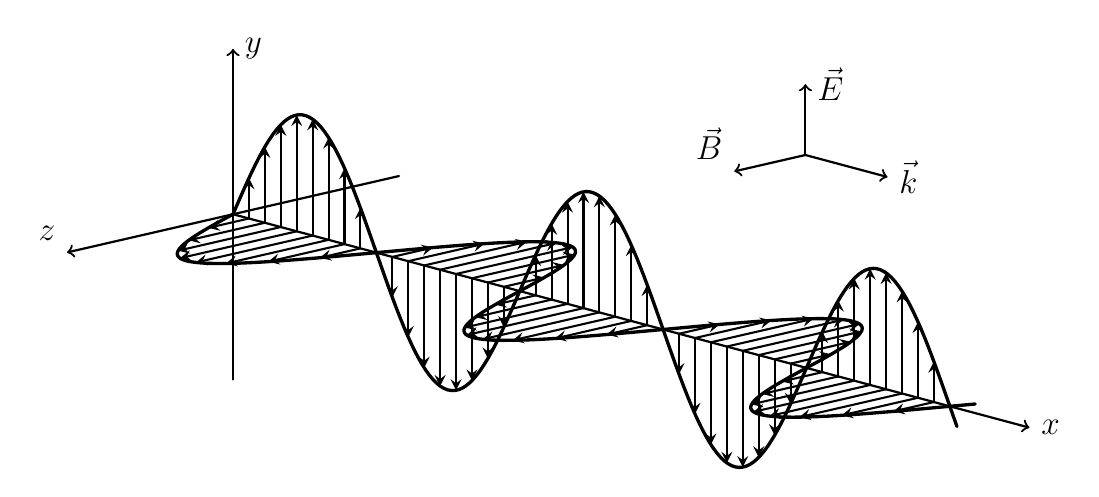
\begin{tikzpicture}[x=(-15:1.2), y=(90:1.0), z=(-150:1.0),
	                    line cap=round, line join=round,
	                    axis/.style={black, thick,->},
	                    vector/.style={>=stealth,->}]
	  \large
	  \def\A{1.5}
	  \def\nNodes{5} % use even number
	  \def\nVectorsPerNode{8}
	  \def\N{\nNodes*40}
	  \def\xmax{\nNodes*pi/2*1.01}
	  \pgfmathsetmacro\nVectors{(\nVectorsPerNode+1)*\nNodes}
	 
	  \def\vE{\mathbf{E}}
	  \def\vB{\mathbf{B}}
	  \def\vk{\mathbf{\hat{k}}}
	 
	  % main axes
	  \draw[axis] (0,0,0) -- ++(\xmax*1.1,0,0) node[right] {$x$};
	  \draw[axis] (0,-\A*1.4,0) -- (0,\A*1.4,0) node[right] {$y$};
	  \draw[axis] (0,0,-\A*1.4) -- (0,0,\A*1.4) node[above left] {$z$};
	 
	  % small axes
	  \def\xOffset{{(\nNodes-2)*pi/2}}
	  \def\yOffset{\A*1.2}
	  \def\zOffset{\A*1.2}
	  \draw[axis] (\xOffset,\yOffset,-\zOffset) -- ++(\A*0.6,0,0) node[right] {$\vec{k}$};
	  \draw[axis] (\xOffset,\yOffset,-\zOffset) -- ++(0,\A*0.6,0) node[right] {$\vec{E}$};
	  \draw[axis] (\xOffset,\yOffset,-\zOffset) -- ++(0,0,\A*0.6) node[above left] {$\vec{B}$};
	 
	  % equation
	  %\node[above right] at (\xOffset,-0.5*\yOffset,4*\zOffset)
	  %  {$\begin{aligned}
	  %    \vE &= \mathbf{E_0}\sin(\vk\cdot\mathbf{x}-c_0t)\\
	  %    \vB &= \mathbf{B_0}\sin(\vk\cdot\mathbf{x}-c_0t)\\
	  %    \end{aligned}$};
	  %\node[below right] at (\xOffset,-0.5*\yOffset,4*\zOffset)
	  %  {$\vE\cdot\vk = 0,\;\; \vB\cdot\vk = 0,\;\; \vB = \frac{1}{c_0}\vk\times\vE$};
	 
	  % waves
	  \draw[very thick,variable=\t,domain=0:\nNodes*pi/2*1.01,samples=\N]
	    plot (\t,{\A*sin(\t*360/pi)},0);
	  \draw[very thick,variable=\t,domain=0:\nNodes*pi/2*1.01,samples=\N]
	    plot (\t,0,{\A*sin(\t*360/pi)});
	 
	  % draw vectors
	  \foreach \k [evaluate={\t=\k*pi/2/(\nVectorsPerNode+1);
	                         \angle=\k*90/(\nVectorsPerNode+1);
	                         \c=(mod(\angle,90)!=0);}]
	              in {1,...,\nVectors}{
	    \if\c1
	      \draw[vector] (\t,0,0) -- ++(0,{\A*sin(2*\angle)},0);
	      \draw[vector] (\t,0,0) -- ++(0,0,{\A*sin(2*\angle)});
	    \fi
	  }
	 
	\end{tikzpicture}
\end{figure}
\FloatBarrier

\section{Energia di un'onda elettromagnetica piana e Vettore di Poynting}

Al campo elettrico e al campo magnetico sono associate delle densità di energia per unità di volume.

\[
	u_e = \frac{1}{2} \varepsilon_0 E^2 \qquad u_m=\frac{1}{2} \frac{B^2}{\mu_0}
\]

Questo fatto si può generalizzare nel caso di campo magnetico ed elettrico variabili nel tempo. La loro presenza comporta l'esistenza di una certa quantità di \textbf{energia distribuita nello spazio} con densità $u$. Per un'onda elettromagnetica avremo una densità di energia per unità di volume pari a:

\begin{align*}
	u = u_e + u_m &= \frac{1}{2} \varepsilon_0 E^2 + \frac{1}{2} \frac{B^2}{\mu_0} \\
	&= \frac{1}{2} \varepsilon_0 B^2 c^2 + \frac{1}{2} \frac{B^2}{\mu_0} \\
	&= \frac{1}{2} \varepsilon_0 B^2 \frac{1}{\mu_0 \varepsilon_0} + \frac{1}{2} \frac{B^2}{\mu_0} \\
	&= \frac{1}{2} \frac{B^2}{\mu_0} + \frac{1}{2} \frac{B^2}{\mu_0} \\
	&= 2u_m = 2u_e \\
	\Aboxed{u = u_e + u_m &= 2u_m = 2u_e}
\end{align*}

Abbiamo scritto una densità di energia istantanea per unità di volume, perché i campi variano nel tempo.
Avendo verificato che un'onda elettromagnetica trasporta dell'energia associata ai due campi, facciamo qualche ragionamento in più sui bilanci energetici dell'interazione tra un'onda elettromagnetica e un sistema. Consideriamo un sistema racchiuso da una superficie $\Sigma$ che interagisca con delle onde elettromagnetiche. Ci possono essere al suo interno delle correnti che eventualmente sono messe in moto da generatori di $fem$, dei campi elettromagnetici e quindi delle onde elettromagnetiche che si propagano e a cui è associata una certa quantità di energia elettromagnetica complessiva:

\[
	\boxed{U = \int_{\tau}(u_e+u_m)d\tau = \int_{\tau}\left[ \frac{1}{2} \vec{D} \cdot \vec{E} + \frac{1}{2} \vec{B} \cdot \vec{H} \right] d\tau}
\]

Si tratta di un'espressione più generale che tiene conto della presenza di eventuali materiali dielettrici e materiali magnetizzati. Tale energia potrà variare nel tempo per vari motivi. I generatori infatti mettono in moto le cariche, ci può essere un flusso di energia causato dalle onde elettromagnetiche che entrano o escono dal sistema trasportando energia o ancora ci può essere dissipazione per effetto Joule. Se andiamo a studiare come tale energia varia, otteniamo:

\begin{equation*}
	\begin{aligned}
		\frac{dU}{dt} &= \int_{\tau}\frac{\partial}{\partial t} \left[ \frac{1}{2} \vec{D} \cdot \vec{E} + \frac{1}{2} \vec{B} \cdot \vec{H} \right] d\tau \\
		&= \int_{\tau} \frac{1}{2} \left[ \frac{\partial \vec{D}}{\partial t} \cdot \vec{E} +\vec{D} \cdot \frac{\partial \vec{E}}{\partial t} + \frac{\partial \vec{B}}{\partial t} \cdot \vec{H} + \vec{B} \cdot \frac{\partial \vec{H}}{\partial t}  \right] d\tau
	\end{aligned}
\end{equation*}

Supponendo che i dielettrici siano omogenei ed isotropi e che i materiali magnetizzati siano di tipo diamagnetico o paramagnetico

\begin{align*}
	\frac{dU}{dt} &= \int_{\tau} \frac{1}{2} \left[ \frac{\partial \vec{D}}{\partial t} \cdot \vec{E} + \varepsilon_0 \varepsilon_r \vec{E} \cdot \frac{\partial \vec{E}}{\partial t} + \frac{\partial \vec{B}}{\partial t} \cdot \vec{H} + \mu_0 \mu_r \vec{H} \cdot \frac{\partial \vec{H}}{\partial t}  \right] d\tau \\
	&= \int_{\tau} \frac{1}{2} \left[ \frac{\partial \vec{D}}{\partial t} \cdot \vec{E} + \vec{E} \cdot \frac{\partial \vec{D}}{\partial t} + \frac{\partial \vec{B}}{\partial t} \cdot \vec{H} + \vec{H} \cdot \frac{\partial \vec{B}}{\partial t}  \right] d\tau \\
	&= \int_{\tau} \left[ \vec{E} \cdot \frac{\partial \vec{D}}{\partial t} + \vec{H} \cdot \frac{\partial \vec{B}}{\partial t}  \right] d\tau \\
	&= \int_{\tau} \left[ \vec{E} \cdot \left( \vec{\nabla} \times \vec{H} -\vec{J}  \right)   + \vec{H} \cdot \left( -\vec{\nabla} \times \vec{E}  \right)    \right] d\tau \tag*{III e IV di Maxwell}\\
	&= \int_{\tau}\left[ \vec{E}\cdot  \vec{\nabla} \times \vec{H} -\vec{H} \cdot \vec{\nabla} \times \vec{E} -\vec{E} \cdot \vec{J}  \right] d\tau
\end{align*}

Si può dimostrare che

\[
	\vec{\nabla} \cdot (\vec{a} \times \vec{b} ) = \vec{b} (\vec{\nabla} \times \vec{a} ) - \vec{a} (\vec{\nabla} \times \vec{b} )
\]

Pertanto:

\begin{equation*}
	\begin{aligned}
		\frac{dU}{dt} &= \int_{\tau} \left[ \vec{\nabla} \cdot \left( \vec{H} \times \vec{E}  \right) - \vec{E} \cdot \vec{J} \right] d\tau \\
		&= \int_{\tau} \left[ - \vec{\nabla} \cdot \underbrace{\left( \vec{E} \times \vec{H}  \right)}_{\vec{S}} - \vec{E} \cdot \vec{J} \right] d\tau
	\end{aligned}
\end{equation*}

Introduciamo una nuova quantità, chiamiamo \textbf{Vettore di Poynting.}

\[
	\boxed{\vec{S} = \vec{E} \times \vec{H}}
\]

Quindi

\begin{equation*}
	\begin{aligned}
		\frac{dU}{dt} &= \int_{\tau} \left[ - \vec{\nabla} \cdot \vec{S} - \vec{E} \cdot \vec{J} \right] d\tau \\
		&= -\int_{\Sigma}\vec{S} \cdot \vec{n} \,dS - \int_{\tau}  \vec{E} \cdot \vec{J} d\tau \\
	\end{aligned}
\end{equation*}

Nel caso di conduttori ohmici possiamo attuare una seconda sostituzione:

\[
	\vec{J} = \sigma (\vec{E} + \vec{E}_m) \implies  \vec{E} = \frac{\vec{J}}{\sigma} - \vec{E}_m = \rho \vec{J} - \vec{E}_m
\]

L'espressione dell'energia diventa quindi:

\[
	\frac{dU}{dt} = -\int_{\Sigma}\vec{S} \cdot \vec{n} \,dS - \int_{\tau}  \left( \rho \vec{J} -\vec{E}_m  \right)   \cdot \vec{J} \, d\tau
\]

\[
	\boxed{\frac{dU}{dt} = -\int_{\Sigma}\vec{S} \cdot \vec{n} \,dS - \int_{\tau} \rho J^2 \, d\tau - \int_{\tau} \vec{J} \cdot \vec{E}_m \, d\tau}
\]

Notiamo che l'ultimo termine ha le dimensioni di una potenza, quindi, trattandosi di una somma, anche gli altri due termini avranno le stesse dimensioni. Possiamo attribuire un significato a questo punto ai contributi rilevati.

\begin{itemize}
	\item Il primo contributo rappresenta la \emph{potenza irradiata verso l'esterno assieme alle onde elettromagnetiche}
	\item Il secondo è l'\emph{energia dissipata per effetto Joule}
	\item Il terzo la \emph{potenza che i generatori danno al sistema} per mantenere le cariche in moto
\end{itemize}

Vediamo come quindi parte dell'energia venga trasformata in calore. A causa dell'ultimo termine tuttavia essa può anche aumentare.
Il bilancio energetico può essere scritto in modo compatto come:

\[
	\frac{dU}{dt} = - W_{oem} - W_J + W_g
\]

Concentriamoci sul primo dei tre contributi di questa sommatoria, che abbiamo detto essere la potenza dissipata durante la propagazione dell'onda. Esso è pari a:

\[
	W_{oem} = \int_{\Sigma} \vec{S} \cdot \vec{n} \,dS
\]

Tale potenza è quindi data dal flusso del vettore di Poynting attraverso la superficie. Il modulo di $\vec{S}$ rappresenta allora l'energia elettromagnetica che per unità di tempo passa attraverso l'unità di superficie ortogonale alla direzione di propagazione. Ecco perché quindi esso prende il nome di \textbf{intensità dell'onda elettromagnetica}.
Nella pratica è importante non tanto calcolare il flusso istantaneo di energia quanto il flusso medio. Il motivo è che la pulsazione delle onde elettromagnetiche è in generale molto elevata $ 10^{15}\,rad/s $ e gli strumenti di misura riescono a determinare soltanto il valor medio dell'energia che li colpisce, non potendo essere sensibili a variazioni così importanti.

Applichiamo questi risultati, validi per una qualsiasi onda elettromagnetica, ad \emph{un'onda piana armonica polarizzata rettilinearmente}. Proviamo a calcolarne il vettore di Poynting.

\begin{align*}
		\vec{H} = \frac{\vec{B}}{\mu_0 \mu_r} \implies \vec{S} &= \vec{E} \times \vec{H} \\
		&=\frac{\vec{E} \times \vec{B}}{\mu_0 \mu_r} \\
		&=\frac{EB\,\vec{u}_z}{\mu_0 \mu_r} \\
		&=\frac{B^2 \,v\,\vec{u}_z}{\mu_0 \mu_r} \\
		&=\frac{B^2}{\mu_0 \mu_r}\vec{v} \\
		&=u\,\vec{v} \\
	\Aboxed{\vec{S} = u\,\vec{v} = \frac{B^2}{\mu_0 \mu_r}\vec{v} &= \varepsilon_0 \varepsilon_r E^2 \vec{v}}
\end{align*}

\begin{figure}[htpb]
	\centering

	\tikzset{every picture/.style={line width=0.75pt}} %set default line width to 0.75pt        

	\begin{tikzpicture}[x=0.75pt,y=0.75pt,yscale=-1,xscale=1]
	%uncomment if require: \path (0,300); %set diagram left start at 0, and has height of 300

	%Straight Lines [id:da7364847646617674] 
	\draw    (192,153) -- (192,69.5) ;
	\draw [shift={(192,66.5)}, rotate = 450] [fill={rgb, 255:red, 0; green, 0; blue, 0 }  ][line width=0.08]  [draw opacity=0] (10.72,-5.15) -- (0,0) -- (10.72,5.15) -- (7.12,0) -- cycle    ;
	%Straight Lines [id:da760698141490767] 
	\draw    (192,153) -- (108.5,153) ;
	\draw [shift={(105.5,153)}, rotate = 360] [fill={rgb, 255:red, 0; green, 0; blue, 0 }  ][line width=0.08]  [draw opacity=0] (10.72,-5.15) -- (0,0) -- (10.72,5.15) -- (7.12,0) -- cycle    ;
	%Straight Lines [id:da3443805156824993] 
	\draw    (192,153) -- (340.4,222.23) ;
	\draw [shift={(343.12,223.5)}, rotate = 205.01] [fill={rgb, 255:red, 0; green, 0; blue, 0 }  ][line width=0.08]  [draw opacity=0] (10.72,-5.15) -- (0,0) -- (10.72,5.15) -- (7.12,0) -- cycle    ;
	%Shape: Boxed Line [id:dp3966841975472175] 
	\draw    (218,135) -- (334.25,189.23) ;
	\draw [shift={(336.97,190.5)}, rotate = 205.01] [fill={rgb, 255:red, 0; green, 0; blue, 0 }  ][line width=0.08]  [draw opacity=0] (10.72,-5.15) -- (0,0) -- (10.72,5.15) -- (7.12,0) -- cycle    ;
	%Straight Lines [id:da8784689277109099] 
	\draw    (243,210.66) -- (304.25,239.23) ;
	\draw [shift={(306.97,240.5)}, rotate = 205.01] [fill={rgb, 255:red, 0; green, 0; blue, 0 }  ][line width=0.08]  [draw opacity=0] (10.72,-5.15) -- (0,0) -- (10.72,5.15) -- (7.12,0) -- cycle    ;

	% Text Node
	\draw (357,225) node    {$\vec{v}$};
	% Text Node
	\draw (210,68) node    {$\vec{E}$};
	% Text Node
	\draw (90,151) node    {$\vec{B}$};
	% Text Node
	\draw (276,246) node    {$\vec{u}_{z}$};
	% Text Node
	\draw (321,163) node    {$\vec{S}$};

	\end{tikzpicture}
\end{figure}
\FloatBarrier

Poiché il campo elettrico di un'onda piana polarizzata può essere pensato come la somma vettoriale di due campi elettrici sfasati, ortogonali tra loro e alla direzione di propagazione, ciascuno trasportante energia elettromagnetica, possiamo calcolar l'intensità media dell'onda per ognuna delle due componenti:

\begin{gather*}
	\vec{E}_y = \vec{E}_{0y}\sin (kx-\omega t)\vec{u}_y \\
	|\vec{S} (t)| = I(t) = \varepsilon_0 \varepsilon_r vE^2 (t) = \varepsilon_0 \varepsilon_r v\,E_{0y}^2 \sin^2 (kx-\omega t) \\
	I_{\text{media}}= I_m = \frac{1}{T}\int_0^T I(t) dt = \varepsilon_0 \varepsilon_r v\,E_{0y}^2 \underbrace{\frac{1}{T} \int_0^T \sin^2 (kx-\omega t)dt}_{= \frac{1}{2}}
\end{gather*}

Quindi

\[
	I_m = \frac{1}{2} \varepsilon_0 \varepsilon_r v\,E_{0y}^2
\]

Per un generico stato di polarizzazione

\[
	\boxed{I_m = \frac{1}{2} \varepsilon_0 \varepsilon_r v \left( E_{0y}^2 + E_{0z}^2 \right)}
\]

\section{Quantità di moto di un'onda elettromagnetica piana}

Per dimostrare che le onde elettromagnetiche trasportano quantità di moto oltre che energia, consideriamo un volume $ \tau  $ in una regione in cui si sta propagando un'onda. Facciamo l'ipotesi che in questo volume siano contenute delle cariche. Sappiamo che la forza agente su una singola carica è data dalla somma di una componente elettrica e di una componente magnetica:

\[
	\vec{F}_{\text{singola carica}} =q\vec{E} +q\vec{v} \times \vec{B}
\]

Se consideriamo un'insieme di cariche, ciascuna di esse si muove di moto casuale, legato all'agitazione termica. Ciò che conta come risultante delle forze è quella parte delle forze di Lorentz che riguarda la componente coordinata del moto delle cariche, e quindi quella velocità di deriva introdotta parlando delle correnti.
A questo punto consideriamo una porzione di materiale. L'onda potrebbe anche non arrestarsi alla superficie, ma attraversarla. Consideriamone un cubetto $ d\tau  $ al cui interno vi sono un numero di cariche $dN$. La forza agente sul cubetto è data da

\[
	d\vec{F} =dN\,q(\vec{E} +\vec{v}_d\times \vec{B}  )
\]

Conviene a questo punto ragionare in termini di forza per unità di volume:

\[
	\vec{f} = \frac{d\vec{F}}{d\tau}=\frac{dN}{d\tau}q(\vec{E} +\vec{v}_d\times \vec{B}  ) = n\,q(\vec{E} +\vec{v}_d\times \vec{B}  )
\]

Possiamo calcolare la potenza dissipata dalla forza all'interno del materiale.

\[
	dW=d\vec{F} \cdot \vec{v}_d
\]

Quella dissipata per unità di volume è data da:

\[
	w=\frac{dW}{d\tau}=\frac{d\vec{F} \cdot \vec{v}_d}{d\tau} = \underbrace{\frac{d\vec{F}}{d\tau}}_{\vec{f}}   \vec{v}_d  = n\,q(\vec{E} +\vec{v}_{d\times \vec{B}}  )\cdot \vec{v}_d = n\,q\,\vec{E} =\vec{J} \cdot \vec{E}
\]

Per i conduttori ohmici abbiamo $w = \vec{J} \cdot \vec{E} =\sigma E^2$.

Si tratta di una potenza istantanea, perché il campo elettrico è oscillante. Se vogliamo lavorare su valori misurabili, si lavora con la potenza media. Notiamo che un onda elettromagnetica interagente con un materiale, può cedere ad esso dell'energia, c'è un assorbimento.

\[
	w_m=\sigma (E^2)_m=\frac{\sigma E_0^2}{2}
\]

Questo non è l'unico effetto che incontriamo. La forza di lorentz è stata scartata perché non compie lavoro, ma non è trascurabile. Il campo $\vec{E}$ pone in moto le cariche e il campo magnetico, vedendole in movimento, applica una forza di Lorentz, diretta nella stessa direzione di propagazione dell'onda. L'onda sta spingendo il materiale. Per comprendere più nel dettaglio cosa accade, ricorriamo al \emph{teorema dell'impulso}.

Grazie ad esso possiamo calcolare la variazione della quantità di moto legata all'azione di una forza variabile nel tempo, in un intervallo T come

\[
	m\vec{v}_f - m\vec{v}_i=\int_{t_i}^{t_f} \vec{F} (t)dt = \vec{I} (t_i,t_f  )
\]

Questo integrale si chiama impulso della forza $\vec{F}$ in $(t_i, t_f)$. Dal momento che siamo interessati all'interazione fra la parte magnetica dell'onda e il materiale, consideriamo solo la componente magnetica della forza per unità di volume:

\[
	\vec{f}_m = n\,q\,\vec{v}_d\times \vec{B} = \vec{J} \times \vec{B} = |\vec{J}|\,|\vec{B}|\vec{u}_x
\]

Possiamo sfruttare la relazione fra campo elettrico e magnetico studiata in precedenza e riscrivere l'espressione in un altro modo:

\[
	\vec{f}_m = |\vec{J}|\,|\vec{B}|\vec{u}_x = \underbrace{\sigma |\vec{E} |}_{|\vec{J}|} |\vec{B} |\vec{u}_x = \sigma E \underbrace{\frac{E}{v}}_B \vec{u}_x = \frac{\sigma E^2}{v}\vec{u}_x
\]

La forza che agisce nella direzione di propagazione dell'onda sarà pari a:

\[
	d\vec{F} = \frac{\sigma E^2}{v}\vec{u}_x \, d\tau
\]

Ci aspettiamo che la forza trasferisca all'oggetto un quantità di moto. Possiamo calcolare la sua variazione su un ciclo $T$ di oscillazione dell'onda con il teorema dell'impulso.

\[
	\frac{\Delta \vec{q}}{T} = \frac{1}{T} \int_0^T d\vec{F} \,dt = d\vec{F}_{\text{media}} =  \frac{\sigma E^2}{v}\vec{u}_x \, d\tau = \frac{w_m\,d\tau}{v}\vec{u}_x
\]

Abbiamo trovato la quantità di moto media ceduta al materiale per unità di tempo e per unità di volume

\[
	\vec{q}_m = \frac{\Delta \vec{q}}{T\,d\tau} = \frac{w_m}{v}\vec{u}_x = \frac{w_m}{v^2}\vec{v}
\]

Abbiamo appreso che quando l'onda elettromagnetica interagisce con il materiale ci sono due effetti:

\begin{itemize}
	\item Dissipazione di energia: l'onda cede energia al materiale perché mette in moto le cariche e compie lavoro.
	\item Trasferimento di quantità di moto: componente magnetica spinge il materiale e le trasferisce una quantità di moto per unità di volume e di tempo direttamente proporzionale alla potenza assorbita per unità di volume.
\end{itemize}

Questo ragionamento attuato in ambito classico, ritorna anche quando si descrive il campo elettromagnetico in termini quantistici. Il campo infatti si può vedere come un'insieme di fotoni, quanti che trasportano energia. In base a quanto visto un fotone deve avere anche una quantità di moto che viene ceduta al materiale, secondo la formula appena trovata. I fotoni quindi pur essendo particelle di massa nulla, hanno anche una quantità i moto.

\textbf{Caso di assorbimento completo dell'onda alla superficie. Processo di radiazione.} Abbiamo ragionato in termini di assorbimento nel volume di un materiale. Ci sono tuttavia delle situazioni in cui l'onda viene assorbita direttamente sulla superficie, senza attraversarla. In tal caso non possiamo ragionare in termini di energia per unità di volume, ma di energia per unità di superficie.
La potenza ceduta alla superficie per unità di superficie è data dal vettore di Poynting. L'intensità media trasferita sarà proprio il modulo di tale vettore.

\[
	I_m = |\vec{S}_m |
\]

La quantità di moto ceduta per unità di tempo unità di superficie sarà pari a: $ \vec{p}_m = \frac{|\vec{S}_m |}{v}\vec{u}_x = \frac{\vec{S}_m}{v}  $. Il vettore di Poynting è diretto secondo la direzione di propagazione dell'onda.

Le dimensioni della quantità di moto saranno date da:

\[
	[\vec{p}_m ] = \frac{[S_m]}{\frac{[L]}{[T]}} = \frac{[S_m][T]}{[L]} = \frac{[W][T]}{[L^2][L]} = \frac{[F][L][T]}{[T][L^2][L]} = \frac{[F]}{[L^2 ]}
\]

Essa ha le dimensioni di una pressione. Viene per questo chiamata pressione di radiazione. Quando un'onda elettromagnetica colpisce una superficie e viene assorbita, la spinge esercitando una pressione. L'effetto è piccolo ma può essere rilevato. Ci sono esperienze di laboratorio in cui si costruiscono dei mulinelli con superfici assorbenti evsi pongono all'interno di una sfera, che così si illumina. C'è chi propone di usare la pressione di radiazione per propulsione spaziale. Costruendo una navicella con una gigantesca vela solare, la pressione di radiazione la spingerebbe senza dover consumare carburante.

\section{Propagazione di onde elettromagnetiche all'interno di un dielettrico}

Siamo interessati a capire come si propagano le onde elettromagnetiche in un materiale dielettrico. Supporremo che esso sia omogeneo e isotropo. Qualunque materiale ha delle proprietà magnetiche, supporremo che si tratti di un materiale o dia o paramagnetico. Valgono allora le seguenti relazioni:

\[
	\vec{D} =\varepsilon_0 \varepsilon_r \vec{E} \qquad \vec{B} =\mu_0 \mu_r \vec{H}
\]

Cominceremo dalle equazioni di Maxwell nella loro forma più generale. Le considereremo sempre in assenza di cariche e correnti nella regione considerata. Sotto queste ipotesi esse sono molto
semplici:

\begin{equation*}
	\begin{aligned}
		&\text{div}\vec{D} =0 \\
		&\text{div}\vec{B} =0 \\
		&\text{rot}\vec{E} = -\frac{\partial \vec{B}}{\partial t} \\
		&\text{rot}\vec{H} = \frac{\partial \vec{D}}{\partial t}
	\end{aligned}
\end{equation*}

Applicando il rotore da entrambe le parti della terza equazione:

\begin{equation*}
	\begin{aligned}
		\vec{\nabla} \times (\vec{\nabla} \times \vec{E} ) &= \vec{\nabla} \times \left( -\frac{\partial \vec{B}}{\partial t}  \right) \\
		\vec{\nabla} ( \underbrace{\vec{\nabla} \cdot \vec{E}}_{=0} )-\nabla^2 \vec{E}  &= - \frac{\partial}{\partial t} ( \vec{\nabla} \times \underbrace{\mu_0 \mu_r \vec{H}}_{\vec{B}} )
	\end{aligned}
\end{equation*}

In quanto $ \text{div}\vec{D} = \text{div}(\varepsilon_0 \varepsilon_r \vec{E} )=\varepsilon_0 \varepsilon_r \,\text{div}\vec{E} = 0 $. Allora continuando i calcoli sulla terza equazione e sostituendo la quarta possiamo scrivere:

\begin{equation*}
	\begin{aligned}
		\nabla^2 \vec{E}  &= \mu_0 \mu_r \frac{\partial}{\partial t} ( \vec{\nabla} \times \vec{H}) \\
		\nabla^2 \vec{E}  &= \mu_0 \mu_r \frac{\partial}{\partial t} \left(\frac{\partial \vec{D}}{\partial t} \right) \\
		\nabla^2 \vec{E}  &= \mu_0 \mu_r \frac{\partial}{\partial t} \left(\frac{\varepsilon_0 \varepsilon_r \partial \vec{E}}{\partial t} \right) \\
		\nabla^2 \vec{E}  &= \mu_0 \mu_r \varepsilon_0 \varepsilon_r \frac{\partial^2 \vec{E}}{\partial t^2} \implies \nabla^2 \vec{E}  - \mu_0 \mu_r \varepsilon_0 \varepsilon_r \frac{\partial^2 \vec{E}}{\partial t^2} = 0\\
	\end{aligned}
\end{equation*}

Abbiamo trovato l'equazione dell'onda, nella forma

\[
	\nabla^2 \xi - \frac{1}{v^2} \frac{\partial^2 \xi}{\partial t^2} =0
\]

Quando abbiamo studiato le onde elettromagnetiche nel vuoto, avevamo detto che $ \frac{1}{c^2}=\mu_0 \varepsilon_0  $. Quello che possiamo dire è che

\[
	\boxed{\frac{1}{v^2}= \mu_0 \varepsilon_0 \mu_r \varepsilon_r =\frac{\mu_r \varepsilon_r}{c^2}}
\]

La velocità delle onde elettromagnetiche nel materiale è diversa

\[
	\boxed{v = \frac{c}{\sqrt{\mu_r \varepsilon_r}}}
\]

In particolare è inferiore alla velocità di propagazione nel vuoto.
Si noti che nei materiali dia e paramagnetici il valore di $\mu_r$ è prossimo all'unità, per cui spesso viene omesso nella espressione di $v$.
Consideriamo solo la parte elettrica in un'onda elettromagnetica piana. Essa si scrive come:

\[
	\vec{E} (x,t)=\vec{E}_0\sin (kx-\omega t) \implies \omega = kc
\]

\begin{figure}[htpb]
	\centering

	% Pattern Info
	 
	\tikzset{
	pattern size/.store in=\mcSize, 
	pattern size = 5pt,
	pattern thickness/.store in=\mcThickness, 
	pattern thickness = 0.3pt,
	pattern radius/.store in=\mcRadius, 
	pattern radius = 1pt}
	\makeatletter
	\pgfutil@ifundefined{pgf@pattern@name@_5m8r8uhee}{
	\pgfdeclarepatternformonly[\mcThickness,\mcSize]{_5m8r8uhee}
	{\pgfqpoint{0pt}{0pt}}
	{\pgfpoint{\mcSize+\mcThickness}{\mcSize+\mcThickness}}
	{\pgfpoint{\mcSize}{\mcSize}}
	{
	\pgfsetcolor{\tikz@pattern@color}
	\pgfsetlinewidth{\mcThickness}
	\pgfpathmoveto{\pgfqpoint{0pt}{0pt}}
	\pgfpathlineto{\pgfpoint{\mcSize+\mcThickness}{\mcSize+\mcThickness}}
	\pgfusepath{stroke}
	}}
	\makeatother
	\tikzset{every picture/.style={line width=0.75pt}} %set default line width to 0.75pt        

	\begin{tikzpicture}[x=0.75pt,y=0.75pt,yscale=-1,xscale=1]
	%uncomment if require: \path (0,300); %set diagram left start at 0, and has height of 300

	%Curve Lines [id:da06465267321472212] 
	\draw [line width=1.5]    (124.5,111.75) .. controls (134.71,111.5) and (134.14,189.5) .. (144.5,189.75) .. controls (154.86,190) and (155.86,112.64) .. (165,112.75) .. controls (174.14,112.86) and (174.43,189.5) .. (185.5,189.25) .. controls (196.57,189) and (195.86,111.21) .. (206,111.25) .. controls (216.14,111.29) and (216.43,189.21) .. (226.5,189.25) .. controls (236.57,189.29) and (236.14,112.07) .. (246.5,112.25) .. controls (256.86,112.43) and (256.43,189.5) .. (267,189.75) .. controls (277.57,190) and (277.29,112.64) .. (287.5,112.75) ;
	%Shape: Rectangle [id:dp2521469075297418] 
	\draw  [draw opacity=0][pattern=_5m8r8uhee,pattern size=6pt,pattern thickness=0.75pt,pattern radius=0pt, pattern color={rgb, 255:red, 222; green, 222; blue, 222}] (337.5,92) -- (427,92) -- (427,207) -- (337.5,207) -- cycle ;
	%Straight Lines [id:da9287130946355424] 
	\draw    (337.5,92) -- (337.5,207) ;
	%Straight Lines [id:da6685712932328518] 
	\draw    (257.5,94) -- (183.5,94) ;
	\draw [shift={(260.5,94)}, rotate = 180] [fill={rgb, 255:red, 0; green, 0; blue, 0 }  ][line width=0.08]  [draw opacity=0] (10.72,-5.15) -- (0,0) -- (10.72,5.15) -- (7.12,0) -- cycle    ;
	%Straight Lines [id:da7983240786429857] 
	\draw    (226,209.25) -- (185.5,209.25) ;
	\draw [shift={(185.5,209.25)}, rotate = 360] [color={rgb, 255:red, 0; green, 0; blue, 0 }  ][line width=0.75]    (0,5.59) -- (0,-5.59)   ;
	\draw [shift={(226,209.25)}, rotate = 360] [color={rgb, 255:red, 0; green, 0; blue, 0 }  ][line width=0.75]    (0,5.59) -- (0,-5.59)   ;

	% Text Node
	\draw (206,219) node    {$\lambda $};
	% Text Node
	\draw (217,56) node   [align=left] {vuoto};
	% Text Node
	\draw (387,56) node   [align=left] {materiale};

	\end{tikzpicture}
\end{figure}
\FloatBarrier

Sappiamo che nel caso di propagazione nel vuoto, la pulsazione $\omega$ è pari a $kc$. In presenza di un dielettrico, sarà pari all'indice $k$ moltiplicato per la velocità di propagazione sopra rilevata. Tuttavia sappiamo che quando un'onda attraversa il materiale, la sua pulsazione non può cambiare perché è legata alla frequenza con cui oscilla nel tempo. Ma il campo elettromagnetico può essere visto come un insieme di fotoni, ciascuno trasportante un'energia $E=hf$. Dal momento che, attraversando un materiale, l'energia di un fotone non varia, anche la frequenza deve rimanere la stessa. Ma se nel passaggio dal vuoto al materiale $\omega$ non può cambiare, deve cambiare $k$. Esso ci da una informazione sulla lunghezza d'onda: $ \lambda=2\pi /k $. Se la velocità di propagazione dal vuoto al materiale diminuisce, essendo $k$ inversamente proporzionale ad essa, $k$ aumenta. Ma se $k$ aumenta, la lunghezza d'onda, per come le due grandezze sono fra di loro legate, diventa più piccola

\[
	\omega = k\,v= k \frac{c}{\sqrt{\mu_r \varepsilon_r}} \implies \boxed{k=\frac{\omega}{c}\sqrt{\mu_r \varepsilon_r}}
\]

Quindi considerando la lunghezza d'onda

\[
	\lambda_{\text{materiale}} = \frac{2\pi}{k_{\text{materiale}}} = \frac{2\pi}{\frac{\omega}{c}\sqrt{\mu_r \varepsilon_r}} = \frac{2\pi c}{\omega \sqrt{\mu_r \varepsilon_r}}
\]

Possiamo a questo punto introdurre una nuova quantità a cui diamo il nome di indice di rifrazione. Esso sarà dato dal rapporto fra la velocità di un'onda elettromagnetica nel vuoto e in un mezzo in cui le onde possono propagarsi, cioè trasparente alle onde elettromagnetiche.
La velocità dell'onda nel materiale si scrive allora come:

\[
	v=\frac{c}{n} \implies \boxed{k=\frac{n\omega}{c}}
\]

E l'indice di rifrazione è dato da:

\[
	\boxed{n=\sqrt{\mu_r \varepsilon_r}}
\]

Per i mezzi trasparenti alle onde elettromagnetiche, $ \mu_r  $ assume valori molto prossimi a $1$:

\[
	\mu_r \simeq 1 \implies n \simeq  \sqrt{\varepsilon_r}
\]

\section{Propagazione di un'onda elettromagnetica in un mezzo dielettrico. Dispersione}

In realtà il problema è molto più complesso di ciò che appare. Il valore di $ \varepsilon_r  $ che compare nella espressione dell'indice di rifrazione non è quello che si misura in regime stazionario (ovvero regime elettrostatico); al contrario esso dipende dalla frequenza $\omega$ dell'onda elettromagnetica (se si considerano onde sinusoidali). Dunque in generale avremo che la velocità di propagazione di un'onda elettromagnetica sinusoidale in un materiale dipende dalla sua frequenza:

\[
	v(\omega)=\frac{c}{n(\omega)}
\]

Questo fenomeno è detto dispersione perché un'onda elettromagnetica composta dalla sovrapposizione di onde di varia frequenza subirà un cambiamento nel corso della propagazione in quanto le sue componenti viaggeranno a differenti velocità. La dispersione è molto importante nel campo delle comunicazioni in fibra ottica.

Si noti che questo non è l'unico effetto che possiamo osservare in un dielettrico; in alcuni casi un'onda elettromagnetica che si propaga subirà una attenuazione; parleremo in tal caso di fenomeno di assorbimento, in quanto l'onda cederà parte della sua energia al materiale. L'intensità di un'onda elettromagnetica diminuisce all'aumentare della distanza di propagazione del materiale.

\begin{figure}[htpb]
	\centering

	\tikzset{every picture/.style={line width=0.75pt}} %set default line width to 0.75pt        

	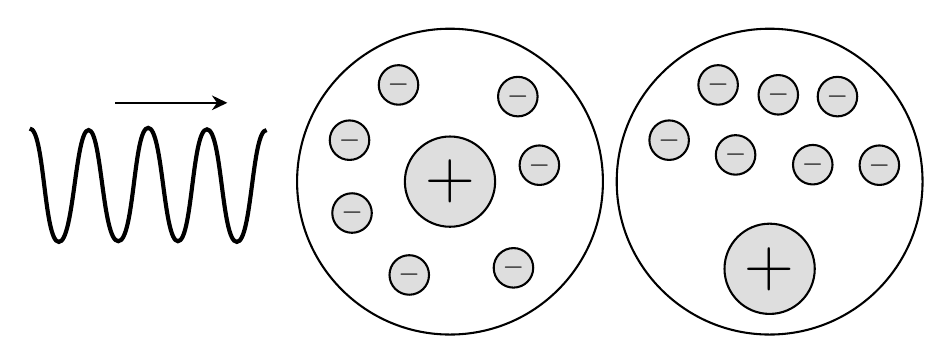
\begin{tikzpicture}[x=0.75pt,y=0.75pt,yscale=-0.7,xscale=0.7]
	%uncomment if require: \path (0,300); %set diagram left start at 0, and has height of 300

	%Shape: Circle [id:dp1413380251931049] 
	\draw   (198.5,168.25) .. controls (198.5,110.12) and (245.62,63) .. (303.75,63) .. controls (361.88,63) and (409,110.12) .. (409,168.25) .. controls (409,226.38) and (361.88,273.5) .. (303.75,273.5) .. controls (245.62,273.5) and (198.5,226.38) .. (198.5,168.25) -- cycle ;
	%Curve Lines [id:da46707183707009703] 
	\draw [line width=1.5]    (14.5,131.75) .. controls (24.71,131.5) and (24.14,209.5) .. (34.5,209.75) .. controls (44.86,210) and (45.86,132.64) .. (55,132.75) .. controls (64.14,132.86) and (64.43,209.5) .. (75.5,209.25) .. controls (86.57,209) and (85.86,131.21) .. (96,131.25) .. controls (106.14,131.29) and (106.43,209.21) .. (116.5,209.25) .. controls (126.57,209.29) and (126.14,132.07) .. (136.5,132.25) .. controls (146.86,132.43) and (146.43,209.5) .. (157,209.75) .. controls (167.57,210) and (167.29,132.64) .. (177.5,132.75) ;
	%Straight Lines [id:da19574424723643502] 
	\draw    (147.5,114) -- (73.5,114) ;
	\draw [shift={(150.5,114)}, rotate = 180] [fill={rgb, 255:red, 0; green, 0; blue, 0 }  ][line width=0.08]  [draw opacity=0] (10.72,-5.15) -- (0,0) -- (10.72,5.15) -- (7.12,0) -- cycle    ;
	%Shape: Circle [id:dp5081045279397389] 
	\draw   (418.5,168.25) .. controls (418.5,110.12) and (465.62,63) .. (523.75,63) .. controls (581.88,63) and (629,110.12) .. (629,168.25) .. controls (629,226.38) and (581.88,273.5) .. (523.75,273.5) .. controls (465.62,273.5) and (418.5,226.38) .. (418.5,168.25) -- cycle ;

	% Text Node
	\draw  [fill={rgb, 255:red, 222; green, 222; blue, 222 }  ,fill opacity=1 ]  (303.75, 168.25) circle [x radius= 31.06, y radius= 31.06]   ;
	\draw (303.75,168.25) node  [font=\Huge]  {$+$};
	% Text Node
	\draw  [fill={rgb, 255:red, 222; green, 222; blue, 222 }  ,fill opacity=1 ]  (268.31, 101.69) circle [x radius= 13.6, y radius= 13.6]   ;
	\draw (268.31,101.69) node    {$-$};
	% Text Node
	\draw  [fill={rgb, 255:red, 222; green, 222; blue, 222 }  ,fill opacity=1 ]  (234.59, 139.72) circle [x radius= 13.6, y radius= 13.6]   ;
	\draw (234.59,139.72) node    {$-$};
	% Text Node
	\draw  [fill={rgb, 255:red, 222; green, 222; blue, 222 }  ,fill opacity=1 ]  (365.27, 156.94) circle [x radius= 13.6, y radius= 13.6]   ;
	\draw (365.27,156.94) node    {$-$};
	% Text Node
	\draw  [fill={rgb, 255:red, 222; green, 222; blue, 222 }  ,fill opacity=1 ]  (236.32, 189.86) circle [x radius= 13.6, y radius= 13.6]   ;
	\draw (236.32,189.86) node    {$-$};
	% Text Node
	\draw  [fill={rgb, 255:red, 222; green, 222; blue, 222 }  ,fill opacity=1 ]  (275.71, 232.49) circle [x radius= 13.6, y radius= 13.6]   ;
	\draw (275.71,232.49) node    {$-$};
	% Text Node
	\draw  [fill={rgb, 255:red, 222; green, 222; blue, 222 }  ,fill opacity=1 ]  (350.44, 109.73) circle [x radius= 13.6, y radius= 13.6]   ;
	\draw (350.44,109.73) node    {$-$};
	% Text Node
	\draw  [fill={rgb, 255:red, 222; green, 222; blue, 222 }  ,fill opacity=1 ]  (347.43, 227.59) circle [x radius= 13.6, y radius= 13.6]   ;
	\draw (347.43,227.59) node    {$-$};
	% Text Node
	\draw  [fill={rgb, 255:red, 222; green, 222; blue, 222 }  ,fill opacity=1 ]  (523.75, 228.25) circle [x radius= 31.06, y radius= 31.06]   ;
	\draw (523.75,228.25) node  [font=\Huge]  {$+$};
	% Text Node
	\draw  [fill={rgb, 255:red, 222; green, 222; blue, 222 }  ,fill opacity=1 ]  (488.31, 101.69) circle [x radius= 13.6, y radius= 13.6]   ;
	\draw (488.31,101.69) node    {$-$};
	% Text Node
	\draw  [fill={rgb, 255:red, 222; green, 222; blue, 222 }  ,fill opacity=1 ]  (454.59, 139.72) circle [x radius= 13.6, y radius= 13.6]   ;
	\draw (454.59,139.72) node    {$-$};
	% Text Node
	\draw  [fill={rgb, 255:red, 222; green, 222; blue, 222 }  ,fill opacity=1 ]  (599.27, 156.94) circle [x radius= 13.6, y radius= 13.6]   ;
	\draw (599.27,156.94) node    {$-$};
	% Text Node
	\draw  [fill={rgb, 255:red, 222; green, 222; blue, 222 }  ,fill opacity=1 ]  (500.32, 149.86) circle [x radius= 13.6, y radius= 13.6]   ;
	\draw (500.32,149.86) node    {$-$};
	% Text Node
	\draw  [fill={rgb, 255:red, 222; green, 222; blue, 222 }  ,fill opacity=1 ]  (529.71, 108.49) circle [x radius= 13.6, y radius= 13.6]   ;
	\draw (529.71,108.49) node    {$-$};
	% Text Node
	\draw  [fill={rgb, 255:red, 222; green, 222; blue, 222 }  ,fill opacity=1 ]  (570.44, 109.73) circle [x radius= 13.6, y radius= 13.6]   ;
	\draw (570.44,109.73) node    {$-$};
	% Text Node
	\draw  [fill={rgb, 255:red, 222; green, 222; blue, 222 }  ,fill opacity=1 ]  (553.43, 156.59) circle [x radius= 13.6, y radius= 13.6]   ;
	\draw (553.43,156.59) node    {$-$};

	\end{tikzpicture}
\end{figure}
\FloatBarrier

Per comprendere l'origine di questi due fenomeni è necessario ricorrere ad un modello semplificato della interazione fra un atomo di un dielettrico ed il campo elettromagnetico. Tenendo conto che gli elettroni sono molto più leggeri dei nuclei atomici, possiamo immaginare che siano i primi ad essere posti in moto da un'onda elettromagnetica incidente sull'atomo, mentre potremo assumere i nuclei sostanzialmente fissi. È utile a questo punto introdurre un modello meccanico dell'atomo, che vediamo come una nube di elettroni intorno ad un nucleo, in cui le forze agenti sull'elettrone sono:

\begin{itemize}
	\item \textbf{una forza di richiamo} (forza di Coulomb) che tende a riportare l'elettrone verso il nucleo quando se ne allontana. L'onda elettromagnetica è composta da campo elettrico e magnetico oscillante che incidono sull'atomo. Il campo elettrico tende a spostare gli elettroni in una direzione e il nucleo in una direzione opposta. Tale forza è in prima approssimazione elastica e la modellizzeremo come:
	\[
		\vec{F}_r= -k\,\vec{r}_e \qquad \vec{r}_e \quad \text{posizione dell'elettrone}
	\]
	\begin{figure}[htpb]
		\centering
		

		\tikzset{every picture/.style={line width=0.75pt}} %set default line width to 0.75pt        

		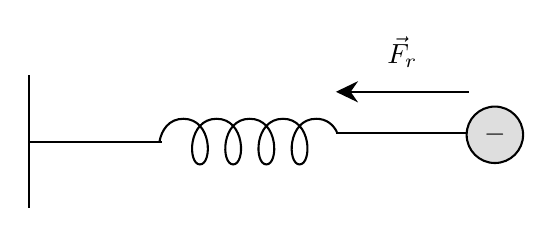
\begin{tikzpicture}[x=0.75pt,y=0.75pt,yscale=-1,xscale=1]
		%uncomment if require: \path (0,300); %set diagram left start at 0, and has height of 300

		%Straight Lines [id:da19276666803521425] 
		\draw    (156,116) -- (156,180) ;
		%Shape: Spring [id:dp8089892542429886] 
		\draw   (219,148) .. controls (220,142.5) and (223.5,137) .. (230.5,137) .. controls (244.5,137) and (244.5,159) .. (238.5,159) .. controls (232.5,159) and (232.5,137) .. (246.5,137) .. controls (260.5,137) and (260.5,159) .. (254.5,159) .. controls (248.5,159) and (248.5,137) .. (262.5,137) .. controls (276.5,137) and (276.5,159) .. (270.5,159) .. controls (264.5,159) and (264.5,137) .. (278.5,137) .. controls (292.5,137) and (292.5,159) .. (286.5,159) .. controls (280.5,159) and (280.5,137) .. (294.5,137) .. controls (299.49,137) and (302.71,139.8) .. (304.5,143.4) ;
		%Straight Lines [id:da10038793636155963] 
		\draw    (220,148) -- (156,148) ;
		%Straight Lines [id:da6277949140980068] 
		\draw    (368,144) -- (304,144) ;
		%Straight Lines [id:da9775807978954678] 
		\draw    (368,124) -- (307,124) ;
		\draw [shift={(304,124)}, rotate = 360] [fill={rgb, 255:red, 0; green, 0; blue, 0 }  ][line width=0.08]  [draw opacity=0] (10.72,-5.15) -- (0,0) -- (10.72,5.15) -- (7.12,0) -- cycle    ;

		% Text Node
		\draw  [fill={rgb, 255:red, 222; green, 222; blue, 222 }  ,fill opacity=1 ]  (380.59, 144.72) circle [x radius= 13.6, y radius= 13.6]   ;
		\draw (380.59,144.72) node    {$-$};
		% Text Node
		\draw (336,105) node    {$\vec{F}_{r}$};

		\end{tikzpicture}
	\end{figure}
	\FloatBarrier

	\item \textbf{una forza dissipativa} che tenga conto della perdita di energia per urti con atomi adiacenti e per emissione di radiazione elettromagnetica, la modellizziamo come una forza di attrito viscoso:
	\[
		\vec{F}_{av} = -b\,\vec{v}_e \qquad \vec{v}_e=\frac{d\vec{r}_e}{dt} \quad \text{velocità dell'elettrone}
	\]
	\item \textbf{una forza che descrive l'interazione tra l'elettrone e l'onda elettromagnetica incidente}, trascureremo gli effetti della componente magnetica (forza di Lorentz) e quindi porremo:
	\[
		\vec{F}_{em} = -e\,\vec{E} (t)
	\]
\end{itemize}

Dove abbiamo tralasciato la dipendenza spaziale di $\vec{E}$ in quanto l'atomo è in una posizione fissa e supporremo che l'elettrone si sposti di poco rispetto alla lunghezza d'onda della radiazione.
A questo punto possiamo applicare il secondo principio della dinamica. L'equazione del moto dell'elettrone sarà:

\begin{equation*}
	\begin{aligned}
		\vec{R} = \vec{F}_r + \vec{F}_{av} + \vec{F}_{em} &= m_e \, \frac{d^2 \vec{r}_e}{dt^2} \\
		-k\,\vec{r}_e -b\,\vec{v}_e -e\,\vec{E} (t) &= m_e \, \frac{d^2 \vec{r}_e}{dt^2} \\
		-\frac{k\,\vec{r}_e}{m_e} - \frac{b\,\vec{v}_e}{m_e} -\frac{e\,\vec{E} (t)}{m_e} &= \frac{d^2 \vec{r}_e}{dt^2} \implies \frac{d^2 \vec{r}_e}{dt^2} + \frac{k\,\vec{r}_e}{m_e} + \frac{b\,\vec{v}_e}{m_e} + \frac{e\,\vec{E} (t)}{m_e} = 0 \\
	\end{aligned}
\end{equation*}

Chiamiamo coefficiente di attrito viscoso, la quantità: $ \gamma = \frac{b}{m_e} $. Sia inoltre $ \omega_0^2 = \frac{k}{m_e}  $. Otteniamo la seguente equazione del moto

\begin{equation}
	\boxed{\frac{\partial^2 \vec{r}_e}{\partial t^2} -\omega_0^2 \,\vec{r}_e + \gamma \frac{\partial \vec{r}_e}{\partial t} + \frac{e}{m_e}\vec{E} (t) = 0}
	\label{eq:oscillatoreAtomico}
\end{equation}

Notiamo che se non ci fosse attrito viscoso otterremmo proprio l'equazione dell'oscillatore armonico

\[
	\frac{\partial^2 \vec{r}_e}{\partial t^2} + \underbrace{\frac{k}{m}}_{\omega_0^2} \vec{r}_e = 0
\]

Grazie a questa osservazione, capiamo che la situazione generale descritta dalla \eqref{eq:oscillatoreAtomico} è quella di un oscillatore atomico di pulsazione propria $ \omega_0  $, la cui oscillazione è smorzata da una forza di attrito viscoso che riassume l'effetto dell'irraggiamento e di una eventuale interazione con gli atomi circostanti.

Risolveremo la \eqref{eq:oscillatoreAtomico} assumendo che l'onda elettromagnetica sia sinusoidale con pulsazione generica $\omega$, dunque ponendo

\[
	\vec{E} (t) = \vec{E}_0 \cos (\omega t)= \frac{\vec{E}_0}{2}[e^{-i\omega t}+e^{i\omega t}  ]  = \frac{\vec{E}_0}{2}e^{-i\omega t} +\frac{\vec{E}_0}{2}e^{i\omega t}
\]

Essendo l'elettrone forzato ad oscillare con la stessa pulsazione di $E(t)$, poniamo analogamente:

\[
	\vec{r}_e = \vec{r}_0 \cos (\omega t) = \frac{\vec{r}_0}{2}[e^{-i\omega t}+e^{i\omega t}  ]  = \frac{\vec{r}_0}{2}e^{-i\omega t} +\frac{\vec{r}_0}{2}e^{i\omega t}
\]

Derivandolo due volte

\begin{equation*}
	\begin{aligned}
		\frac{d\vec{r}_e}{dt} &= -i\omega \frac{\vec{r}_0}{2}e^{-i\omega t} + c.c. \\
		\frac{d^2 \vec{r}_e}{dt^2} &= (-i\omega)^2 \frac{\vec{r}_0}{2}e^{-i\omega t} + c.c. = - \frac{\omega^2\vec{r}_0}{2}e^{-i\omega t} + c.c.
	\end{aligned}
\end{equation*}

Sostituendo questa espressione nell'equazione \eqref{eq:oscillatoreAtomico}

\begin{gather*}
	\left[ -\frac{\omega^2 \vec{r}_0}{2} +\frac{\omega^2 \vec{r}_0}{2} - \frac{i\omega \gamma \vec{r}_0}{2} + \frac{e}{m_e}\frac{\vec{E}_0}{2} \right] e^{-i\omega t} + \\
	+ \left[ -\frac{\omega^2 \vec{r}_0}{2} +\frac{\omega^2 \vec{r}_0}{2} - \frac{i\omega \gamma \vec{r}_0}{2} + \frac{e}{m_e}\frac{\vec{E}_0}{2} \right] e^{i\omega t} =0
\end{gather*}

Perché l'equazione sia sodisfatta, è necessario che il termine nelle parentesi quadre si annulli.

\begin{equation*}
	\begin{aligned}
		-\omega^2 \vec{r}_0 + \omega_0 ^2 \vec{r}_0 - i\gamma \omega \vec{r}_0 + \frac{e}{m_e}\vec{E}_0 &=0 \\
		\vec{r}_0[\omega_0^2 -\omega^2  - i\gamma \omega] + \frac{e}{m_e} \vec{E}_0 &=0 \\
		\vec{r}_0 = -\frac{e\vec{E}_0}{[\omega_0^2 -\omega^2  - i\gamma \omega]m_e} \\
		\vec{r}_e(t) = \frac{\vec{r}_0}{2} (e^{-i\omega t}+e^{i\omega t}  ) &= -\frac{e\vec{E}_0}{2[\omega_0^2 -\omega^2  - i\gamma \omega]m_e} (e^{-i\omega t}+e^{i\omega t}  )
	\end{aligned}
\end{equation*}

Abbiamo così trovato la soluzione della \eqref{eq:oscillatoreAtomico}, che rappresenta l'equazione del moto dell'elettrone oscillante in un atomo, quando eccitato da un'onda elettromagnetica. Poiché l'elettrone oscilla a causa del campo $\vec{E}$, l'atomo presenterà un momento di dipolo oscillante pari a: $ \vec{p} = -e \vec{r}_e  $. In un materiale con $N$ atomi per unità di volume, definiamo il vettore polarizzazione come:

\begin{equation*}
	\begin{aligned}
		\vec{P} = N\vec{p} =-Ne\,\vec{r}_e &= -N e \left( -\frac{\vec{r}_0}{2}(e^{-i\omega t}+e^{i\omega t}) \right) \\
		&= \frac{N\,e^2 \vec{E}_0}{2[\omega_0^2-\omega^2 -i\gamma \omega]m_e}(e^{-i\omega t}+e^{i\omega t}) \\
		&= \frac{\vec{P}_0}{2} (e^{-i\omega t}+e^{i\omega t})
	\end{aligned}
\end{equation*}

Sarà questo il vettore polarizzazione $\vec{P}$ in un mezzo dielettrico composto da atomi identici con densità per unità di volume $N$.
Ricordiamo la relazione $ \vec{P} = \varepsilon_0 (\varepsilon_r -1)\vec{E}  $
Essa era stata introdotta per i campi elettrostatici. Estendendola anche ai campi (e di conseguenza alla polarizzazione) oscillanti nel tempo, avremo:

\begin{gather*}
	\vec{P}_0 = \frac{Ne^2 \,\vec{E}_0}{[\omega_0^2-\omega^2 -i\gamma \omega]m_e} = \varepsilon_0 \left[ \varepsilon_r (\omega) -1 \right] \vec{E}_0 \\
	\boxed{\varepsilon_r (\omega) = 1 + \frac{Ne^2}{m_e\,\varepsilon_0\,[\omega_0^2-\omega^2 -i\gamma \omega]}}
\end{gather*}

Moltiplicando nominatore e denominatore per il complesso coniugato:

\[
	\varepsilon_r (\omega) = 1 + \frac{Ne^2 \left[ (\omega_0^2 -\omega^2) + i\gamma\omega  \right]}{m_e\,\varepsilon_0\,\left[ (\omega_0^2 -\omega^2)^2 +\gamma^2 \omega^2 \right]}
\]

Possiamo definire un indice di rifrazione complesso che sarà la radice quadrata della quantità appena ricavata.

\[
	n = \sqrt{\varepsilon_r (\omega)}
\]

Per calcolarla possiamo ricorrere a delle approssimazioni basata sull'idea che il dielettrico considerato sia rarefatto. In tal caso:

\[
	n=\sqrt{\varepsilon_r (\omega)} = \sqrt{1 + \underbrace{\frac{Ne^2 \left[ (\omega_0^2 -\omega^2) + i\gamma\omega  \right]}{m_e\,\varepsilon_0\,\left[ (\omega_0^2 -\omega^2)^2 +\gamma^2 \omega^2 \right]}}_{\to 0}}
\]

In una situazione di questo tipo, in cui abbiamo una funzione della forma

\[
	f(x) = \sqrt{1+x} \qquad x\to 0
\]

Possiamo attuare la seguente approssimazione:

\[
	f(x) = 1 + \frac{x}{2} + o(x)
\]

L'indice di rifrazione sarà allora dato da:

\[
	n \simeq 1 + \frac{Ne^2 \left[ (\omega_0^2 -\omega^2) + i\gamma\omega  \right]}{2\,m_e\,\varepsilon_0\,\left[ (\omega_0^2 -\omega^2)^2 +\gamma^2 \omega^2 \right]} = n_R + i\,n_I
\]

Con

\begin{align*}
	n_R &= 1 + \frac{Ne^2}{2m_e\,\varepsilon_0}\frac{\omega_0^2 -\omega^2}{\left[ (\omega_0^2 -\omega^2)^2 +\gamma^2 \omega^2 \right]} \\
	n_I &= 1 + \frac{Ne^2}{2m_e\,\varepsilon_0}\frac{\gamma \omega}{\left[ (\omega_0^2 -\omega^2)^2 +\gamma^2 \omega^2 \right]}
\end{align*}

Per comprendere il significato di quanto trovato, rianalizziamo l'equazione delle onde, che aveva comportato nel caso di onde piane la soluzione:

\begin{equation*}
	\begin{aligned}
		\vec{E} (x,t) &= \frac{\vec{E}_0}{2}e^{i(kx-\omega t)} + \frac{\vec{E}_0}{2}e^{-i(kx-\omega t)} \qquad k = \frac{n\omega}{c} \\
		&=\frac{\vec{E}_0}{2}e^{i\left( \frac{\omega}{c}n_Rx + \frac{\omega}{c}n_Ix - \omega t   \right)} + c.c.
	\end{aligned}
\end{equation*}

La sostituzione operata su $k$ proviene dalle seguenti considerazioni:

\[
	\omega = kv \qquad k = \frac{\omega}{v} = \frac{\omega}{c/n} = \frac{n\omega}{c} = \frac{\omega}{c} [n_R + i\,n_I]
\]
\emph{Nota}: per semplicità di scrittura indichiamo con $c.c.$ il complesso coniugato del termine appena precedente.
Sarà possibile scrivere l'onda nella forma:

\begin{equation*}
	\begin{aligned}
		\vec{E} (x,t) &= \frac{\vec{E}_0}{2}e^{i\left[ \frac{\omega}{c}n_R x-\omega t \right]} e^{-\frac{\omega}{c}n_I x} + c.c. \\
		&= \frac{\vec{E}_0}{2} e^{i[k_R(\omega) x - \omega t ]} e^{-\alpha(\omega)\,x} + c.c.
	\end{aligned}
\end{equation*}

abbiamo posto:

\begin{gather*}
	k_R(\omega) = \frac{\omega}{c} n_R(\omega) \\
	\alpha (\omega) = \frac{\omega}{c} n_I(\omega)
\end{gather*}

l'espressione del campo elettrico può allora essere scritta come:

\[
	\boxed{\vec{E} (x,t) = \vec{E}_0 e^{-\alpha x} \cos [k_R(\omega)x-\omega t]}
\]

Dove compare un'espressione più generale del numero d'onda $k$ ed un termine esponenziale decrescente

\[
	\vec{E}_0\,e^{-\alpha x}
\]

Che dunque comporta un'alterazione dell'onda durante la propagazione. Si vede che la sua intensità diminuisce esponenzialmente con la distanza, indicando un assorbimento di energia da parte del dielettrico. Anche l'intensità media, proporzionale al quadrato dell'ampiezza, diminuisce progressivamente con legge esponenziale:

\[
	I(x) = I(0)\,e^{-2\alpha x} = I(0)\,e^{-\beta x}
\]

\begin{figure}[htpb]
	\centering

	\tikzset{every picture/.style={line width=0.75pt}} %set default line width to 0.75pt        

	\begin{tikzpicture}[x=0.75pt,y=0.75pt,yscale=-1,xscale=1]
	%uncomment if require: \path (0,300); %set diagram left start at 0, and has height of 300

	%Shape: Axis 2D [id:dp8573669816086147] 
	\draw  (174,225) -- (481.5,225)(194.5,51) -- (194.5,241) (474.5,220) -- (481.5,225) -- (474.5,230) (189.5,58) -- (194.5,51) -- (199.5,58)  ;
	%Curve Lines [id:da0876937084718834] 
	\draw [line width=1.5]    (194.5,74) .. controls (205.5,177) and (208.5,218) .. (274.5,221) .. controls (340.5,224) and (366.5,221) .. (407.5,222) ;

	% Text Node
	\draw (168,53) node    {$I( x)$};
	% Text Node
	\draw (495,223) node    {$x$};

	\end{tikzpicture}
\end{figure}
\FloatBarrier

$\beta$ prende il nome di \textbf{coefficiente di assorbimento}. Il suo inverso, $\frac{1}{\beta}$, è la \textbf{lunghezza di assorbimento} e ha il solito significato: dopo una distanza $\frac{1}{\beta}$ nel dielettrico l'intensità si è ridotta al valore $I(0)e^{-1}$.
In conclusione, la dispersione durante la propagazione dell'onda nel mezzo è descritta completamente dalla parte reale $n_R$ dell'indice di rifrazione complesso, mentre la parte immaginaria $n_I$ determina il coefficiente di assorbimento ed è quindi legata alla diminuzione dell'intensità dell'onda.

\begin{figure}[htpb]
	\centering

	\tikzset{every picture/.style={line width=0.75pt}} %set default line width to 0.75pt        

	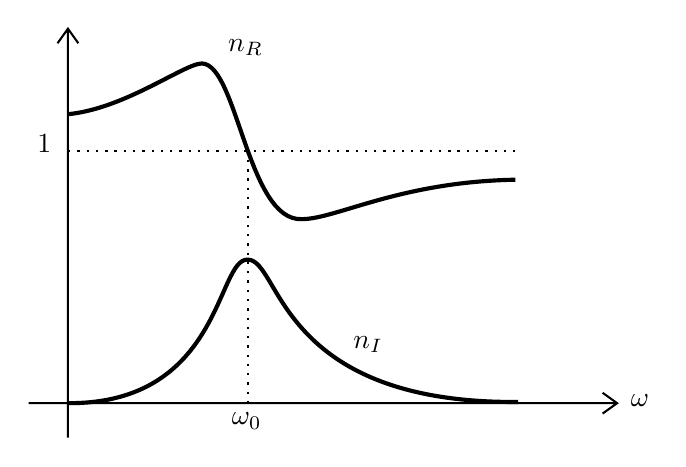
\begin{tikzpicture}[x=0.75pt,y=0.75pt,yscale=-1,xscale=1]
	%uncomment if require: \path (0,300); %set diagram left start at 0, and has height of 300

	%Shape: Axis 2D [id:dp7607986096735857] 
	\draw  (173.5,244.41) -- (457,244.41)(192.4,64) -- (192.4,261) (450,239.41) -- (457,244.41) -- (450,249.41) (187.4,71) -- (192.4,64) -- (197.4,71)  ;
	%Curve Lines [id:da5227641534353398] 
	\draw [line width=1.5]    (192.67,105.17) .. controls (220.33,102.33) and (248.5,80.75) .. (257,80.75) .. controls (274,81.25) and (279,156.75) .. (305,155.75) .. controls (321.67,155.75) and (352,137.75) .. (408,136.75) ;
	%Curve Lines [id:da08841698827363254] 
	\draw [line width=1.5]    (192.57,244.41) .. controls (266.5,244.75) and (264,174.75) .. (279,175.25) .. controls (295,175.25) and (293,244.75) .. (409.33,243.83) ;
	%Straight Lines [id:da9091818157433591] 
	\draw  [dash pattern={on 0.84pt off 2.51pt}]  (279,122.75) -- (279,244.75) ;
	%Straight Lines [id:da9890017011677661] 
	\draw  [dash pattern={on 0.84pt off 2.51pt}]  (408,122.75) -- (193,122.75) ;

	% Text Node
	\draw (468,243) node    {$\omega $};
	% Text Node
	\draw (181,119.5) node    {$1$};
	% Text Node
	\draw (278,73) node    {$n_{R}$};
	% Text Node
	\draw (278.5,253) node    {$\omega _{0}$};
	% Text Node
	\draw (337,216) node    {$n_{I}$};

	\end{tikzpicture}
\end{figure}
\FloatBarrier

In corrispondenza del massimo assorbimento c'è anche un cambiamento di velocità.

\section{Equazioni di Maxwell in presenza di sorgenti. Potenziali elettrodinamici}

Finora ci siamo occupati delle equazioni di Maxwell e della loro risoluzione in assenza di sorgenti. Vogliamo quindi ora occuparci del caso più generale in cui sono presenti sorgenti variabili nel tempo. Questa situazione si può riscrivere tramite i potenziali elettrodinamici. Ipotizziamo di essere nel vuoto. Le equazioni saranno date da:

\begin{align}
	\text{div}\vec{E} &=\frac{\rho (t)}{\varepsilon_0} \label{eq:max1}\\
	\text{rot}\vec{E} &= -\frac{\partial \vec{B}}{\partial t} \label{eq:max2} \\
	\text{div}\vec{B} &= 0 \label{eq:max3}\\
	\text{rot}\vec{B} &= \mu_0 \left[ \vec{J} (t) + \varepsilon_0 \frac{\partial \vec{E}}{\partial t}  \right] \label{eq:max4}
\end{align}

Si dimostra dall'equazione \eqref{eq:max3} che possiamo sempre scrivere il campo magnetico $\vec{B}$ come il rotore di un certo potenziale vettore $\vec{A}$, $ \vec{B} = \text{rot}\vec{A} $.
Applicando poi l'operatore divergenza e si trova:

\[
	\text{div}\vec{B} = \text{div}(\text{rot}\vec{A} ) = \vec{\nabla} \cdot (\vec{\nabla} \times \vec{A} ) = 0
\]

Sostituendo l'espressione di $\vec{B}$ nella seconda equazione:

\[
	\vec{\nabla} \times \vec{E} = -\frac{\partial}{\partial t}(\underbrace{\vec{\nabla} \times \vec{A}}_{\vec{B}} ) = \vec{\nabla} \times \left( -\frac{\partial \vec{A}}{\partial t}  \right) \implies \vec{\nabla} \times \left( \vec{E} +\frac{\partial \vec{A}}{\partial t}  \right) =0
\]

L'ultima espressione afferma che il vettore fra parentesi è conservativo e dunque è possibile introdurre un potenziale scalare $V$ tale che

\[
	\vec{E} +\frac{\partial \vec{A}}{\partial t} = - \vec{\nabla} V
\]

Quindi abbiamo

\[
	\boxed{\vec{B} = \vec{\nabla} \times \vec{A} \qquad \vec{E} =-\vec{\nabla} V-\frac{\partial \vec{A}}{\partial t}}
\]

Questi potenziali li abbiamo definiti partendo da due equazioni che non dipendono dalle sorgenti, quindi valgono in qualsiasi situazione. Vogliamo sostituire questi due potenziale nelle equazioni rimanenti. Nella \eqref{eq:max1}:

\begin{equation*}
	\begin{aligned}
		\vec{\nabla} \cdot \vec{E} =\vec{\nabla} \cdot \left( -\vec{\nabla} V-\frac{\partial \vec{A}}{\partial t}  \right) &= \frac{\rho (t)}{\varepsilon_0} \\
		- \nabla^2 V - \vec{\nabla} \cdot \left( \frac{\partial \vec{A}}{\partial t}  \right) &= \frac{\rho (t)}{\varepsilon_0} \implies
		\nabla^2 V + \vec{\nabla} \cdot \frac{\partial \vec{A}}{\partial t} &= -\frac{\rho (t)}{\varepsilon_0}
	\end{aligned}
\end{equation*}

Se fossimo al regime stazionario, ritorneremmo all'equazione di Poisson già incontrata. A questo punto dall'equazione \eqref{eq:max4} ricaviamo:

\begin{equation*}
	\begin{aligned}
		\vec{\nabla} \times \underbrace{\vec{\nabla} \times \vec{A}}_{\vec{B}}  &= \mu_0 \left[ \vec{J} (t) + \varepsilon_0 \frac{\partial}{\partial t} \overbrace{\left(-\vec{\nabla} V - \frac{\partial \vec{A}}{\partial t}\right)}^{\vec{E}}   \right] \\
		\vec{\nabla} (\vec{\nabla} \cdot \vec{A} ) - \nabla^2 \vec{A} &= \mu_0 \vec{J} (t) + \underbrace{\mu_0 \varepsilon_0}_{1/c^2} \left( -\frac{\partial \vec{\nabla} V}{\partial t} -\frac{\partial^2 \vec{A}}{\partial t^2}  \right)  \\
		\nabla^2 \vec{A} -\frac{1}{c^2}\frac{\partial^2 \vec{A}}{\partial t^2} -\frac{1}{c^2}\frac{\partial \vec{\nabla} V}{\partial t} - \vec{\nabla} (\vec{\nabla} \cdot \vec{A} ) &= -\mu_0 \vec{J} (t) \\
		\nabla^2 \vec{A} -\frac{1}{c^2}\frac{\partial^2 \vec{A}}{\partial t^2} - \vec{\nabla} \left(\frac{1}{c^2}\frac{\partial V}{\partial t} + \vec{\nabla} \cdot \vec{A} \right) &= -\mu_0 \vec{J} (t) \\
	\end{aligned}
\end{equation*}

Abbiamo così ottenuto due equazioni differenziali nei soli potenziali $\vec{A}$ e $V$ che dipendono dalle sorgenti note. Si osservi che il numero di equazioni scalari e di funzioni incognite è il medesimo. Tuttavia le equazioni non sono disaccoppiate, per disaccoppiarle si sfrutta una libertà nella scelta delle funzioni incognite $\vec{A}$ e $V$ detta \textbf{invarianza di gauge}, che pur trasformando $\vec{A}$ e $V$ in nuove funzioni $\vec{A'}$ e $V'$, mantiene inalterati i valori di $\vec{E}$ e di $\vec{B}$ a cui siamo in realtà interessati.

Infatti, scegliendo una funzione $f$ qualsiasi purché derivabile, poniamo di ottenere nuovi potenziali a partire dai precedenti con le trasformazioni:

\[
	\boxed{\vec{A} \to \vec{A}' = \vec{A} +\vec{\nabla} \vec{f} \qquad V\to V' = V-\frac{\partial f}{\partial t}}
\]

Pertanto le trasformazioni proposte non alternano i valori di $\vec{E}$ e di $ \vec{B}  $, ma possono consentire di riscrivere le equazioni dei potenziali in forma opportuna. Sceglieremo allora una opportuna trasformazione che comporti il seguente legame:

\[
	\boxed{\frac{1}{c^2}\frac{\partial V'}{\partial t} + \vec{\nabla} \cdot \vec{A'} = 0}
\]

Questa condizione è anche nota come \textbf{condizione di Lorentz}. Pur non dimostrandone la fattibilità, osserviamo che esiste una opportuna funzione f che consente di scrivere tale relazione. Dalla condizione di Lorentz, le due equazioni nei potenziali diventano:

\begin{equation}
	\boxed{\nabla^2 \vec{A} -\frac{1}{c^2}\frac{\partial^2 \vec{A}}{\partial t^2} = -\mu_0 \vec{J} (t)}
\end{equation}

Ricordiamo ora che:

\[
	\frac{1}{c^2}\frac{\partial V'}{\partial t} + \vec{\nabla} \cdot \vec{A'} = 0 \implies  \vec{\nabla} \cdot \vec{A} = - \frac{1}{c^2}\frac{\partial V}{\partial t}
\]

Quindi:

\begin{equation*}
	\begin{aligned}
		\nabla^2 V + \vec{\nabla} \cdot \frac{\partial \vec{A}}{\partial t} &= -\frac{\rho (t)}{\varepsilon_0} \\
		\nabla^2 V + \frac{\partial}{\partial t} (\vec{\nabla} \cdot \vec{A}) &= -\frac{\rho (t)}{\varepsilon_0} \\
		\nabla^2 V + \frac{\partial}{\partial t} \left( - \frac{1}{c^2}\frac{\partial V}{\partial t} \right)   &= -\frac{\rho (t)}{\varepsilon_0} \\
	\end{aligned}
\end{equation*}

\begin{equation}
	\boxed{\nabla^2 V  - \frac{1}{c^2}\frac{\partial^2 V}{\partial t^2} = -\frac{\rho (t)}{\varepsilon_0}}
\end{equation}

In tal modo le due equazioni si disaccoppiano, perché non compaiono più i due potenziali nella stessa equazione. Se fossimo in regime stazionario le equazioni diventerebbero semplicemente:

\[
	\nabla^2 V  = -\frac{\rho (t)}{\varepsilon_0} \qquad \nabla^2 \vec{A} = -\mu_0 \vec{J} (t)
\]

La prima è l'equazione di Poisson e la seconda è stata ricavata in magnetostatica. Quindi le due equazioni comprendono tutti i casi e si possono estendere anche a quello stazionario. Avendo introdotto l'operatore d'alembertiano, possiamo riscrivere le due equazioni semplicemente come:

\[
	\boxed{\left\{ \begin{array}{l}
		 	\Box \vec{A} = -\mu_0 \vec{J} (t) \\
		 	\Box \vec{V} = -\frac{\rho (t)}{\varepsilon_0}
		\end{array} \right.}
\]

La soluzione delle due equazioni è anche essa simile a quanto trovato nel caso stazionario, ma tiene conto della variazione temporale delle sorgenti.
Supponiamo di avere un certo volume $\tau$. In ogni cubetto $d\tau$ vi sono cariche e correnti che variano nel tempo.

\begin{figure}[htpb]
	\centering

	\tikzset{every picture/.style={line width=0.75pt}} %set default line width to 0.75pt        

	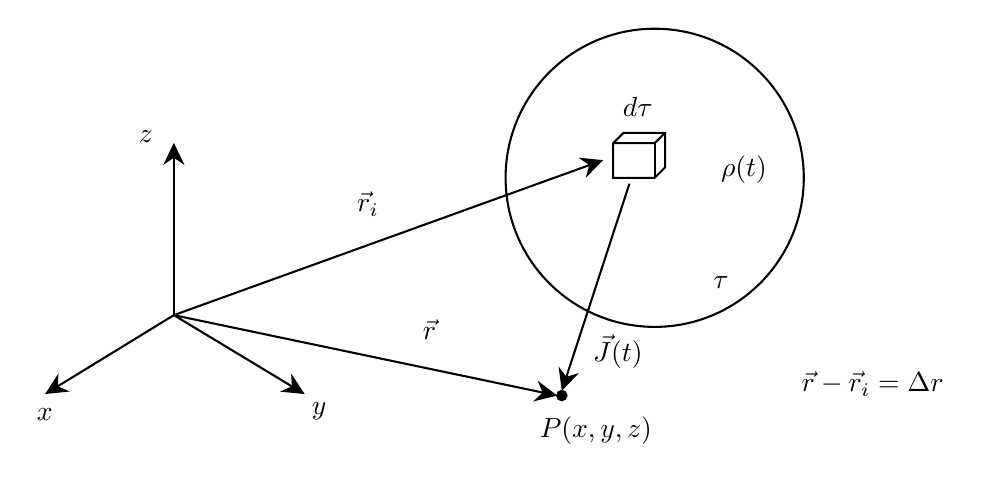
\begin{tikzpicture}[x=0.75pt,y=0.75pt,yscale=-1,xscale=1]
	%uncomment if require: \path (0,300); %set diagram left start at 0, and has height of 300

	%Straight Lines [id:da6797463639029115] 
	\draw    (216.5,185.67) -- (216.5,105.67) ;
	\draw [shift={(216.5,102.67)}, rotate = 450] [fill={rgb, 255:red, 0; green, 0; blue, 0 }  ][line width=0.08]  [draw opacity=0] (10.72,-5.15) -- (0,0) -- (10.72,5.15) -- (7.12,0) -- cycle    ;
	%Straight Lines [id:da15998144999629993] 
	\draw    (216.5,185.67) -- (276.93,222.12) ;
	\draw [shift={(279.5,223.67)}, rotate = 211.1] [fill={rgb, 255:red, 0; green, 0; blue, 0 }  ][line width=0.08]  [draw opacity=0] (10.72,-5.15) -- (0,0) -- (10.72,5.15) -- (7.12,0) -- cycle    ;
	%Straight Lines [id:da31848190328869985] 
	\draw    (216.5,185.67) -- (157.06,222.1) ;
	\draw [shift={(154.5,223.67)}, rotate = 328.5] [fill={rgb, 255:red, 0; green, 0; blue, 0 }  ][line width=0.08]  [draw opacity=0] (10.72,-5.15) -- (0,0) -- (10.72,5.15) -- (7.12,0) -- cycle    ;
	%Shape: Circle [id:dp1661340389317938] 
	\draw  [fill={rgb, 255:red, 0; green, 0; blue, 0 }  ,fill opacity=1 ] (401.17,224.42) .. controls (401.17,223.17) and (402.17,222.17) .. (403.42,222.17) .. controls (404.66,222.17) and (405.67,223.17) .. (405.67,224.42) .. controls (405.67,225.66) and (404.66,226.67) .. (403.42,226.67) .. controls (402.17,226.67) and (401.17,225.66) .. (401.17,224.42) -- cycle ;
	%Straight Lines [id:da9318394165074981] 
	\draw    (216.5,185.67) -- (420.51,112.02) ;
	\draw [shift={(423.33,111)}, rotate = 520.15] [fill={rgb, 255:red, 0; green, 0; blue, 0 }  ][line width=0.08]  [draw opacity=0] (10.72,-5.15) -- (0,0) -- (10.72,5.15) -- (7.12,0) -- cycle    ;
	%Straight Lines [id:da5083602993568179] 
	\draw    (216.5,185.67) -- (398.23,223.8) ;
	\draw [shift={(401.17,224.42)}, rotate = 191.85] [fill={rgb, 255:red, 0; green, 0; blue, 0 }  ][line width=0.08]  [draw opacity=0] (10.72,-5.15) -- (0,0) -- (10.72,5.15) -- (7.12,0) -- cycle    ;
	%Straight Lines [id:da6962376677301336] 
	\draw    (436,122.33) -- (404.35,219.31) ;
	\draw [shift={(403.42,222.17)}, rotate = 288.08] [fill={rgb, 255:red, 0; green, 0; blue, 0 }  ][line width=0.08]  [draw opacity=0] (10.72,-5.15) -- (0,0) -- (10.72,5.15) -- (7.12,0) -- cycle    ;
	%Shape: Circle [id:dp25731616548756575] 
	\draw   (376.33,119.5) .. controls (376.33,79.83) and (408.49,47.67) .. (448.17,47.67) .. controls (487.84,47.67) and (520,79.83) .. (520,119.5) .. controls (520,159.17) and (487.84,191.33) .. (448.17,191.33) .. controls (408.49,191.33) and (376.33,159.17) .. (376.33,119.5) -- cycle ;
	%Shape: Cube [id:dp047324299810165726] 
	\draw   (428.17,102.83) -- (433.17,97.83) -- (453.17,97.83) -- (453.17,114.5) -- (448.17,119.5) -- (428.17,119.5) -- cycle ; \draw   (453.17,97.83) -- (448.17,102.83) -- (428.17,102.83) ; \draw   (448.17,102.83) -- (448.17,119.5) ;

	% Text Node
	\draw (154.33,233.67) node    {$x$};
	% Text Node
	\draw (286.5,232.17) node    {$y$};
	% Text Node
	\draw (203,99.67) node    {$z$};
	% Text Node
	\draw (430.47,203.4) node    {$\vec{J}( t)$};
	% Text Node
	\draw (339.67,192.83) node    {$\vec{r}$};
	% Text Node
	\draw (310,132.17) node    {$\vec{r}_{i}$};
	% Text Node
	\draw (419.83,241.33) node    {$P( x ,y,z)$};
	% Text Node
	\draw (439.97,85.27) node    {$d\tau $};
	% Text Node
	\draw (480.17,170.07) node    {$\tau $};
	% Text Node
	\draw (491.17,115.67) node    {$\rho ( t)$};
	% Text Node
	\draw (553.17,218.87) node    {$\vec{r} -\vec{r}_{i} =\Delta r$};

	\end{tikzpicture}
\end{figure}
\FloatBarrier

Si dimostra che in tale situazione le soluzioni alle due equazioni sono date da:

\begin{gather*}
	\boxed{V(\vec{r},t) = \int_{\tau}\frac{\rho (\vec{r'}, t - \frac{\Delta r}{c})}{4\pi \varepsilon_0 \, \Delta r}d\tau} \\
	\boxed{\vec{A} (\vec{r},t) = \int_{\tau}\frac{\mu_0 \vec{J} (\vec{r'}, t - \frac{\Delta r}{c})}{4\pi \, \Delta r}d\tau} \\
\end{gather*}

I potenziali così ricavati mantengono la stessa struttura del caso stazionario, ma le sorgenti vanno valutate non nello stesso istante t in cui valutiamo i potenziali nel punto $P(r)$, bensì in un istante precedente $ t'=t-\frac{\Delta \vec{r}}{c} $, per tener conto del ritardo di propagazione delle informazioni dalla sorgente al punto $P$. Per questo motivo tali quantità sono anche dette \emph{potenziali ritardati}, si noti che quanto esposto rappresenta solo un integrale particolare delle equazioni per i potenziali; l'integrale generale si ottiene come combinazione lineare di quello particolare con la soluzione delle rispettive equazioni omogenee, che corrispondono alla propagazione di onde elettromagnetiche in assenza di sorgenti.

\section{Campo elettromagentico prodotto da un bipolo elettrico oscillante}

Consideriamo il caso di un dipolo che oscilla sinusoidalmente con pulsazione $\omega$. Vorremmo determinare, sfruttando le equazioni dei potenziali ritardati, l'andamento della radiazione elettromagnetica emessa dal dipolo.

\begin{figure}[htpb]
	\centering

	\tikzset{every picture/.style={line width=0.75pt}} %set default line width to 0.75pt        

	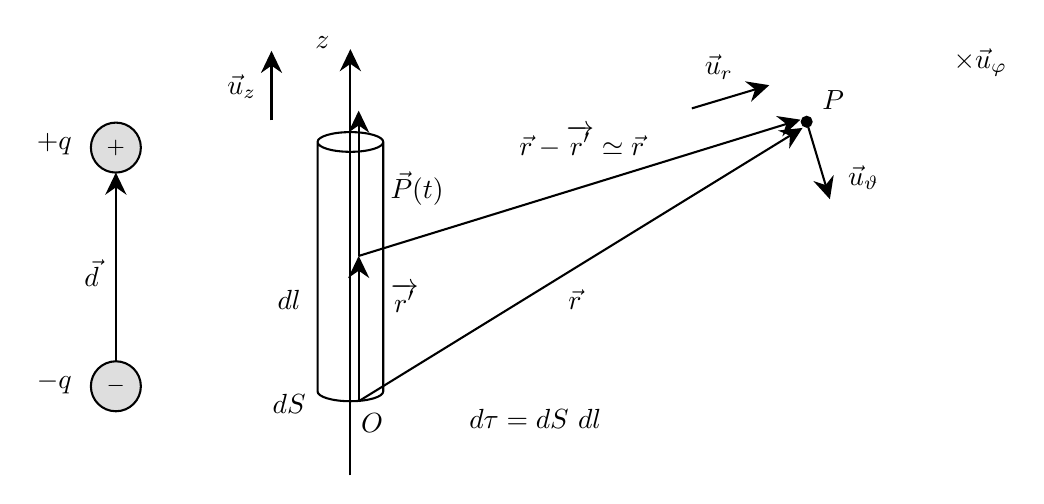
\begin{tikzpicture}[x=0.75pt,y=0.75pt,yscale=-1,xscale=1]
	%uncomment if require: \path (0,300); %set diagram left start at 0, and has height of 300

	%Straight Lines [id:da05818592277158685] 
	\draw    (240.5,257) -- (240.5,54.67) ;
	\draw [shift={(240.5,51.67)}, rotate = 450] [fill={rgb, 255:red, 0; green, 0; blue, 0 }  ][line width=0.08]  [draw opacity=0] (10.72,-5.15) -- (0,0) -- (10.72,5.15) -- (7.12,0) -- cycle    ;
	%Straight Lines [id:da3710797089764373] 
	\draw    (244.5,221.33) -- (455.78,91.24) ;
	\draw [shift={(458.33,89.67)}, rotate = 508.38] [fill={rgb, 255:red, 0; green, 0; blue, 0 }  ][line width=0.08]  [draw opacity=0] (10.72,-5.15) -- (0,0) -- (10.72,5.15) -- (7.12,0) -- cycle    ;
	%Shape: Can [id:dp6034508492628499] 
	\draw   (256.33,96.42) -- (256.33,216.58) .. controls (256.33,219.21) and (249.24,221.33) .. (240.5,221.33) .. controls (231.76,221.33) and (224.67,219.21) .. (224.67,216.58) -- (224.67,96.42) .. controls (224.67,93.79) and (231.76,91.67) .. (240.5,91.67) .. controls (249.24,91.67) and (256.33,93.79) .. (256.33,96.42) .. controls (256.33,99.04) and (249.24,101.17) .. (240.5,101.17) .. controls (231.76,101.17) and (224.67,99.04) .. (224.67,96.42) ;
	%Straight Lines [id:da3866371667239994] 
	\draw    (244.5,221.33) -- (244.5,154.33) ;
	\draw [shift={(244.5,151.33)}, rotate = 450] [fill={rgb, 255:red, 0; green, 0; blue, 0 }  ][line width=0.08]  [draw opacity=0] (10.72,-5.15) -- (0,0) -- (10.72,5.15) -- (7.12,0) -- cycle    ;
	%Straight Lines [id:da20551356813850896] 
	\draw    (244.5,151.33) -- (244.5,84.33) ;
	\draw [shift={(244.5,81.33)}, rotate = 450] [fill={rgb, 255:red, 0; green, 0; blue, 0 }  ][line width=0.08]  [draw opacity=0] (10.72,-5.15) -- (0,0) -- (10.72,5.15) -- (7.12,0) -- cycle    ;
	%Straight Lines [id:da2652861406077569] 
	\draw    (244.5,151.33) -- (454.47,86.55) ;
	\draw [shift={(457.33,85.67)}, rotate = 522.85] [fill={rgb, 255:red, 0; green, 0; blue, 0 }  ][line width=0.08]  [draw opacity=0] (10.72,-5.15) -- (0,0) -- (10.72,5.15) -- (7.12,0) -- cycle    ;
	%Straight Lines [id:da35178094374328306] 
	\draw    (405,80.25) -- (439.46,69.92) ;
	\draw [shift={(442.33,69.06)}, rotate = 523.3199999999999] [fill={rgb, 255:red, 0; green, 0; blue, 0 }  ][line width=0.08]  [draw opacity=0] (10.72,-5.15) -- (0,0) -- (10.72,5.15) -- (7.12,0) -- cycle    ;
	%Shape: Circle [id:dp8287369725898297] 
	\draw  [fill={rgb, 255:red, 0; green, 0; blue, 0 }  ,fill opacity=1 ] (457.95,86.67) .. controls (457.95,85.35) and (459.02,84.29) .. (460.33,84.29) .. controls (461.65,84.29) and (462.71,85.35) .. (462.71,86.67) .. controls (462.71,87.98) and (461.65,89.05) .. (460.33,89.05) .. controls (459.02,89.05) and (457.95,87.98) .. (457.95,86.67) -- cycle ;
	%Straight Lines [id:da5074134243029063] 
	\draw    (460.33,86.67) -- (470.66,121.13) ;
	\draw [shift={(471.52,124)}, rotate = 253.32] [fill={rgb, 255:red, 0; green, 0; blue, 0 }  ][line width=0.08]  [draw opacity=0] (10.72,-5.15) -- (0,0) -- (10.72,5.15) -- (7.12,0) -- cycle    ;
	%Straight Lines [id:da272551315978391] 
	\draw    (202.5,86) -- (202.5,55.52) ;
	\draw [shift={(202.5,52.52)}, rotate = 450] [fill={rgb, 255:red, 0; green, 0; blue, 0 }  ][line width=0.08]  [draw opacity=0] (10.72,-5.15) -- (0,0) -- (10.72,5.15) -- (7.12,0) -- cycle    ;

	% Text Node
	\draw (227,48.67) node    {$z$};
	% Text Node
	\draw  [fill={rgb, 255:red, 222; green, 222; blue, 222 }  ,fill opacity=1 ]  (127.51, 214.13) circle [x radius= 12.04, y radius= 12.04]   ;
	\draw (127.51,214.13) node  [font=\footnotesize]  {$-$};
	% Text Node
	\draw (251,232) node    {$O$};
	% Text Node
	\draw (211,222.67) node    {$dS$};
	% Text Node
	\draw (211,172.67) node    {$dl$};
	% Text Node
	\draw (272.67,118.67) node    {$\vec{P}( t)$};
	% Text Node
	\draw (266.67,171.67) node    {$\overrightarrow{r'}$};
	% Text Node
	\draw (348.67,172.33) node    {$\vec{r}$};
	% Text Node
	\draw (352,96.33) node    {$\vec{r} -\overrightarrow{r'} \simeq \vec{r}$};
	% Text Node
	\draw (418,60.33) node    {$\vec{u}_{r}$};
	% Text Node
	\draw (473.14,76.05) node    {$P$};
	% Text Node
	\draw (544,58.33) node    {$\times \vec{u}_{\varphi }$};
	% Text Node
	\draw (487.71,113.76) node    {$\vec{u}_{\vartheta }$};
	% Text Node
	\draw (329.57,229.81) node    {$d\tau =dS\ dl$};
	% Text Node
	\draw (188.14,69.81) node    {$\vec{u}_{z}$};
	% Text Node
	\draw  [fill={rgb, 255:red, 222; green, 222; blue, 222 }  ,fill opacity=1 ]  (127.51, 99.13) circle [x radius= 12.04, y radius= 12.04]   ;
	\draw (127.51,99.13) node  [font=\footnotesize]  {$+$};
	% Text Node
	\draw (97.86,97.52) node    {$+q$};
	% Text Node
	\draw (97.86,212.52) node    {$-q$};
	% Text Node
	\draw (115.86,159.52) node    {$\vec{d}$};
	% Connection
	\draw    (127.51,202.09) -- (127.51,114.17) ;
	\draw [shift={(127.51,111.17)}, rotate = 450] [fill={rgb, 255:red, 0; green, 0; blue, 0 }  ][line width=0.08]  [draw opacity=0] (10.72,-5.15) -- (0,0) -- (10.72,5.15) -- (7.12,0) -- cycle    ;

	\end{tikzpicture}
\end{figure}
\FloatBarrier

Considereremo a tal fine il dipolo come un elemento di volume $d\tau$ al cui interno il vettore polarizzazione sia diretto lungo l'asse $z$ e vari nel tempo secondo la relazione:

\[
	\vec{P} (t) = P_0\sin (\omega t)\vec{u}_z
\]

Possiamo a tal punto determinare la corrente di polarizzazione che scorre nell'elemento di volume come:

\[
	\vec{J}_p = \frac{\partial \vec{P}}{\partial t} = P_0\omega \cos (\omega t) \vec{u}_z
\]

Inseriremo questa corrente nell'espressione del potenziale ritardato $\vec{A}(\vec{r},t)$, dove $\vec{r}$ individua la posizione del punto $P$ in cui valutare tale vettore. Otterremo:

\[
	\vec{A}(\vec{r}, t) = \int_{\tau}\frac{\mu_0 \vec{J}_p(\vec{r'},t-\frac{\Delta r}{c})}{4\pi \Delta r} d\tau
\]

Con $ \Delta \vec{r} = \vec{r} - \vec{r'} $ e $ \vec{r'}$ la posizione dell'elemento di corrente. Ponendo l'origine del sistema di coordinate in corrispondenza del dipolo stesso, avremo:

\[
	\vec{r'} \simeq 0 \implies  \Delta \vec{r} = \vec{r} - \vec{r'} \simeq \vec{r}
\]

Inoltre risulta che:

\[
	\vec{J}_pd\tau = \frac{\partial \vec{P} \, d\tau}{\partial t} = \frac{\partial \vec{p}}{\partial t}
\]

Pertanto risulterà che:

\[
	\vec{A} (\vec{r},t) = \frac{\mu_0 \dot{\vec{p}}(t-\frac{r}{c})}{4\pi r} = \frac{\mu_0 \dot{p}(t-\frac{r}{c})}{4\pi r} \vec{u}_z \qquad \left( \dot{\vec{p}} = \frac{\partial \vec{p}}{\partial t}  \right)
\]

Dato che:

\[
	\vec{p} (t) = p_0 \sin (\omega t) \vec{u}_z \implies \dot{\vec{p}} = p_0\omega \cos (\omega t) \vec{u}_z
\]

Si ha:

\[
	\boxed{\vec{A} (\vec{r},t) = \frac{\mu_0}{4\pi} \frac{p_0 \omega}{r} \cos \left[ \omega\left( t-\frac{r}{c} \right)   \right]  \vec{u}_z}
\]
$\vec{A}$ è in tutti i punti dello spazio diretto come l'asse $z$.
Potremo poi determinare il potenziale scalare ritardato $V$ impiegando la condizione di Lorentz:

\[
	\vec{\nabla} \cdot \vec{A} + \frac{1}{c^2}\frac{\partial V}{\partial t} =0 \implies  \frac{\partial V}{\partial t} = - c^2 \vec{\nabla} \cdot \vec{A} = - c^2 \frac{\partial A_z}{\partial z}
\]

Essendo le altre componenti di $\vec{A}$ nulle. Partendo da questo punto si può dimostrare che:

\begin{gather*}
	V(t)=\int \frac{\partial V}{\partial t} \partial + \text{costante}\\
	\Downarrow\\
	V(\vec{r},t) = \frac{z}{4\pi \varepsilon_0 r}\left[ \frac{p(t-\frac{r}{c})}{r^2} + \frac{\dot{p}(t-\frac{r}{c})}{cr}\right]
\end{gather*}

Che nel nostro caso specifico diverrà:

\[
	\boxed{V(\vec{r},t) = \frac{z}{4\pi \varepsilon_0 r}\left[ \frac{p_0\sin [\omega(t-\frac{r}{c})]}{r^2} + \frac{p_0\omega\cos [\omega(t-\frac{r}{c})]}{cr}\right]}
\]

Nel caso di un dipolo che non cambia forma, avevamo trovato che in regime stazionario il potenziale assume questa forma:

\[
	V(r) = \frac{\vec{p} \cdot \vec{u}_r}{4\pi \varepsilon_0 r^2} = \frac{p_0\vec{u}_r\cdot r\,\vec{u}_r}{4\pi \varepsilon_0 r^3} = \frac{p_0\vec{u}_r\cdot \vec{r}}{4\pi \varepsilon_0 r^3} = \frac{p_0z}{4\pi \varepsilon_0 r^3}
\]

Notiamo quindi che un dipolo statico con momento di dipolo $ p_0  $ darebbe vita ad un potenziale elettrostatico coincidente solo con la prima parte dell'espressione di $V(\vec{r}, t)$ pur di sostituire il momento di dipolo dipolo $p(t)$ con il momento di dipolo $p_0 $. Dunque nel caso tempo variante la struttura del potenziale scalare cambia notevolmente. Mentre il primo pezzo ha al denominatore $r^2$, il secondo ha $r$. Le due parti non hanno lo stesso andamento nel tempo, ma l'ultima decresce più lentamente.

A partire dalle espressioni trovate per $\vec{A}$ e per $V$ è possibile determinare i campi $\vec{E}$ e $\vec{B}$ delle onde elettromagnetiche prodotte, mediante le relazioni:

\[
	\vec{B} =\text{rot}\vec{A} \qquad \vec{E} =-\text{grad}V - \frac{\partial \vec{A}}{\partial t}
\]

Tenendo conto solo dei termini che decrescono più lentamente con la distanza, si troverà allora che, a grande distanza dal dipolo:

\begin{gather*}
	\vec{B} \sim \frac{\mu_0}{4\pi} \frac{\sin \vartheta \ddot{p}(t-\Delta r/t)}{rc}\vec{u}_{\varphi}\\
	\vec{E} \sim \frac{1}{4\pi \varepsilon_0}\frac{\sin \vartheta \ddot{p}(t-r/t)}{rc^2} \vec{u}_\vartheta
\end{gather*}

Nel caso specifico:

\begin{gather*}
	p=p_0\sin (\omega t)\\
	\ddot{p} = - \omega^2 p_0\sin (\omega t)\\
	\ddot{p} (t-r/c) = -\omega^2 p_0\sin \left[ \omega\left( t-\frac{r}{c} \right)   \right] = \omega^2 p_0\sin \left( \frac{\omega}{c}r-\omega t \right)
\end{gather*}

Ottenendo allora:

\begin{gather*}
	\vec{B} = \frac{B_0\sin \vartheta \sin (kr-\omega t)}{r}\vec{u}_{\varphi}\\
	\vec{E} = \frac{B_0c\sin \vartheta \sin (kr-\omega t)}{r}\vec{u}_\vartheta
\end{gather*}

Caratteristico di un'\textbf{onda sferica}. Si tratta di un onda che si propaga in tutte le direzioni, non su un asse. L'ampiezza dell'onda non è costante ma allontanandosi dal dipolo diminuisce sempre di più.
è utile osservare che il vettore di Poynting è dato da:

\[
	\vec{S} =\vec{E} \times \vec{H} = \frac{\vec{E} \times \vec{B}}{\mu_0} = \frac{p_0^2 \omega^4 \sin^2 \vartheta \sin^2 [\omega(t-r/c)]}{16\pi^2 \varepsilon_0 c^3  r^2} \vec{u}_r
\]

E notando che il valor medio su un ciclo ottico del termine tempovariante è pari a $\frac{1}{2} $ si otterrà alla fine:

\[
	\vec{S}_m = \frac{P_0^2 \omega^4 \sin^2 \vartheta}{32\pi^2 r^2 c^3 \varepsilon_0} \vec{u}_r = I_m\vec{u}_r
\]

Dove per $I_m $ intendiamo l'intensità media in funzione della distanza dal dipolo e dell'angolo $\vartheta $ che $ \vec{u}_r $ forma con $p$.
Se studiamo il bipolo come se fosse un \textbf{antenna}, le onde elettromagnetiche non hanno intensità costante in tutte le direzioni: sono più intense in direzione perpendicolare a quella dell'oscillazione. Nella direzione parallela al dipolo, non c'è campo magnetico.

\begin{figure}[htpb]
	\centering

	\tikzset{every picture/.style={line width=0.75pt}} %set default line width to 0.75pt        

	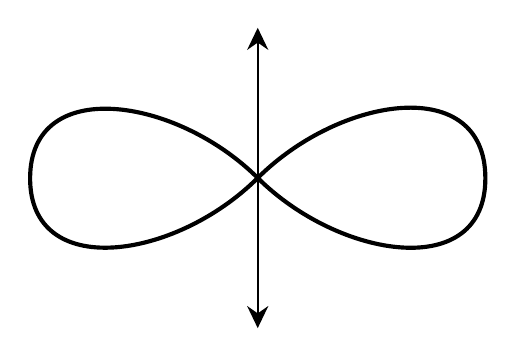
\begin{tikzpicture}[x=0.75pt,y=0.75pt,yscale=-1,xscale=1]
	%uncomment if require: \path (0,300); %set diagram left start at 0, and has height of 300

	%Straight Lines [id:da42412084017493457] 
	\draw    (260.5,189.69) -- (260.5,50.98) ;
	\draw [shift={(260.5,47.98)}, rotate = 450] [fill={rgb, 255:red, 0; green, 0; blue, 0 }  ][line width=0.08]  [draw opacity=0] (10.72,-5.15) -- (0,0) -- (10.72,5.15) -- (7.12,0) -- cycle    ;
	\draw [shift={(260.5,192.69)}, rotate = 270] [fill={rgb, 255:red, 0; green, 0; blue, 0 }  ][line width=0.08]  [draw opacity=0] (10.72,-5.15) -- (0,0) -- (10.72,5.15) -- (7.12,0) -- cycle    ;
	%Shape: Polygon Curved [id:ds9861847736168488] 
	\draw  [line width=1.5]  (370.17,120.33) .. controls (370.33,170.67) and (299.67,159.33) .. (260.5,120.33) .. controls (221.33,81.33) and (151,70.67) .. (150.83,120.33) .. controls (150.66,170) and (220.67,160) .. (260.5,120.33) .. controls (300.33,80.67) and (370.01,70) .. (370.17,120.33) -- cycle ;

	\end{tikzpicture}
\end{figure}
\FloatBarrier

Il calcolo della potenza $W$ irradiata dall'onda generata dal dipolo oscillante attraverso una superficie sferica $\Sigma$ centrata nel dipolo ed avente raggio $r$ è pari a:

\begin{align*}
	W_{oem} &= \int_{\Sigma} \vec{S}_m\cdot \vec{n} dS = \int_{\Sigma}\vec{S}_m\cdot \vec{u}_rdS\\
	&= \int_{\Sigma} \frac{p_0^2 \omega^4 \sin^2 \vartheta}{32\pi^2 r^2 \varepsilon_0 c^3} \cdot 2\pi r\sin \vartheta rd\vartheta  \\
	&= \frac{p_0^2 \omega^4}{16\pi \varepsilon_0 c^3} \underbrace{\int_0^{\pi} \sin^3 \vartheta d\vartheta}_{4/3} \\
	&= \frac{p_0^2 \omega^4}{12\pi \varepsilon_0 c^3}
\end{align*}

Che a parità di frequenza ed ampiezza del dipolo non dipende dal raggio della superficie prescelto. Pertanto, al fine di conservare la potenza irradiata, i campi $\vec{E}$ e $\vec{B}$ devono decrescere come $1/r$ per compensare l'aumento dell'area con $r$.
Come ultima osservazione notiamo che dalla formula generale di $\vec{E}$ e $\vec{B}$ a grandi distanze otteniamo

\[
	\vec{S} = \frac{\sin^2 \vartheta \left[ \ddot{p}\left( t-\frac{r}{c} \right)   \right]^2}{16\pi^2 \varepsilon_0 c^3 r^2} \vec{u}_r
\]

Qualora il dipolo oscillante fosse composto da una carica $-q$ in quiete ed una $+q$ in moto accelerato, otterremo:

\[
	\vec{p} = q\vec{d} \implies \ddot{\vec{p}}=\frac{d^2 \vec{p}}{dt^2} = q\frac{d^2 \vec{d}}{dt^2} = q\vec{a}
\]

Dove $a$ è l'accelerazione della carica positiva. Pertanto possiamo dalla formula precedente ottenere l'espressione dell'intensità di radiazione emessa da una carica $q$ in moto accelerato:

\[
	\vec{S} = \frac{\sin^2 \vartheta\,  q^2 a^2 \left( t-\frac{r}{c} \right) ^2}{16\pi^2 \varepsilon_0 c^3 r^2} \vec{u}_r
\]

Una carica in moto accelerato emette onde elettromagnetiche e la potenza di questa emissione va con il quadrato della distanza. Se $ a $ è costante:

\[
	W_{oem} = \frac{q^2 a^2}{6\pi \varepsilon_0 c^3} \qquad \text{Formula di Larmor}
\]